\section{Naključne konstrukcije}
Cilj poglavja je generiranje Ramanujanovih grafov na računalniku. Uporabili bomo najenostavnejši algoritem: generiramo naključen \(d\)-regularen graf in izračunamo njegovo spektralno vrzel. Če je dovolj velika, je naš graf Ramanujanov, če pa je premajhna, graf zavržemo in generiramo nov graf, dokler ne dobimo takega, ki ima dovolj veliko spektralno vrzel. Računanje lastnih vrednosti grafa je zelo enostavno, zato si bomo podrobneje ogledali le algoritem za učinkovito generiranje naključnih regularnih grafov.

S pomočjo dobljenega algoritma si lahko ogledamo nekaj lastnosti grafov. Zanima nas velikost spektralne vrzeli v odvisnosti od števila vozlišč in delež Ramanujanov grafov. Če je ta delež dovolj velik, je naš algoritem učinkovit in lahko enostavno generiramo Ramanujanove grafe. Velikost povprečne spektralne vrzeli pa nam pove, kako daleč je poljuben graf od tega, da je Ramanujanov; Ramanujanovi grafi imajo sicer zanimive matematične lastnosti, v praksi bi se pa morda kdaj zadovoljili že z grafom, ki je ``približno'' Ramanujanov.

\subsection{Algoritmi za generiranje regularnih grafov}
Generiranje regularnih grafov je netrivialen problem. Težava pri večini pristopov je, da ne moremo povezav dodajati iterativno in imeti zagotovljeno, da na koncu dobimo regularen graf. Oglejmo si to na enostavnem primeru.

\begin{primer}
    Za primer bomo poskusili generirati \(2\)-regularen graf na štirih vozliščih. Tak graf seveda obstaja, na primer cikel \(C_4\). Naš algoritem bo sledeč: izberemo naključni dve vozlišči, ki imata stopnjo manjšo od \(2\) in ju povežemo. To ponavljamo, dokler ne dobimo grafa, ki je \(2\)-regularen.

    Začnemo s praznim grafom, ki ima vozlišča \(\{1, 2, 3, 4\}\). Izberemo naključni dve vozlišči, recimo \(1\) in \(2\), in ju povežemo. Nato izberemo vozlišči \(2\) in \(3\) in ju povežemo, zatem pa še \(3\) in \(1\) in ju povežemo. Sedaj imamo \(3\) vozlišča stopnje \(2\) in enega stopnje \(0\). Ob vsaki točki smo izbrali vozlišči, ki imata stopnjo manjšo od \(2\), algoritem pa se ne more zaključiti, saj smo prišli do točke, ko vozlišča \(4\) ne moremo povezati z nobenim vozliščem, ki ima stopnjo manjšo od \(2\).
\end{primer}

V tem primeru je bil problem, da ne moremo povezati vozlišča s samim seboj, lahko pa bi se zgodilo tudi, da imamo dve vozlišči stopnje \(d-1\), ki pa ju ne moremo povezati, saj sta že povezani. Obstaja enostaven način, kako lahko rešimo to težavo: če algoritma ne moremo zaključiti, graf zavržemo in začnemo znova. Z malo optimizacije nas to prinese do algoritma \ref{enakomerno-nakljucni-pocasi}, ki generira kandidate, in algoritma \ref{enakomerno-nakljucni-pomozno}, ki ponavlja klice na algoritem \ref{enakomerno-nakljucni-pocasi}, dokler ne dobimo veljavnega regularnega grafa \cite{kim-vu-regularni}. Algoritem \ref{enakomerno-nakljucni-pomozno} bomo uporabljali tudi pri vseh ostalih pristopih za generiranje regularnih grafov.

\algnewcommand\algorithmicto{\textbf{to}}
\algnewcommand\algorithmicin{\textbf{in}}
\algnewcommand\algorithmicforeach{\textbf{for each}}
\algrenewtext{For}[3]{\algorithmicfor\ #1 $\gets$ #2\ \algorithmicto\ #3\ \algorithmicdo}
\algdef{S}[FOR]{ForEach}[2]{\algorithmicforeach\ #1\ \algorithmicin\ #2\ \algorithmicdo}

\begin{algorithm}[t]
    \caption{Generiranje naključnih regularnih grafov}
    \label{enakomerno-nakljucni-pomozno}
    \raggedright
    \textbf{Vhod:} Števili \(n, d \in \mathbb N\). \\
    \textbf{Izhod:} Sosednostna matrika \(A\) \(d\)-regularnega grafa na \(n\) vozliščih.
    \begin{algorithmic}[1]
        \Function{generiraj}{$n$, $d$}
        \While{True}
        \State \(A \gets \Call{generiraj-pomozno}{n, d}\)
        \If{\Call{je-regularen-graf}{$A$, $d$}}
        \State \Return $A$
        \EndIf
        \EndWhile
        \EndFunction
    \end{algorithmic}
\end{algorithm}

\begin{algorithm}[t]
    \caption{Generiranje naključnih regularnih grafov}
    \label{enakomerno-nakljucni-pocasi}
    \raggedright
    \textbf{Vhod:} Števili \(n, d \in n, d \in \mathbb N\). \\
    \textbf{Izhod:} Sosednostna matrika \(A\) \(d\)-regularnega grafa na \(n\) vozliščih.
    \begin{algorithmic}[1]
        \Function{generiraj-pomozno}{$n$, $d$}
        \For{$i$}{$0$}{$n-1$}
        \For{$j$}{$0$}{$d-1$}
        \State \(krajisce[i\cdot n + j] \gets i\) \Comment{Ustvarimo \(d\) kopij vsakega vozlišča.}
        \EndFor
        \EndFor
        \State \(krajisce' \gets \Call{shuffle}{krajisce}\)
        \State \(A \gets\) ničelna matrika velikosti \(n \times n\)
        \For{$i$}{$0$}{$n\cdot d - 1$}
        \State \(A_{krajisce[i], krajisce'[i]} \gets 1\)
        \State \(A_{krajisce'[i], krajisce[i]} \gets 1\)
        \EndFor
        \State \Return $A$
        \EndFunction
    \end{algorithmic}
\end{algorithm}

Algoritem \ref{enakomerno-nakljucni-pocasi} je sicer pravilen, vendar pa je zelo počasen. Velikokrat se zgodi, da moramo ponovno generirati graf, še posebej za velike \(d\), zaradi česar postane neuporaben za generiranje večjih grafov. Izkaže se, da je verjetnost generiranja regularnega grafa \(O(e^{-\frac{d^2}{4}})\) \cite{STEGER_WORMALD_1999}, kar se zelo hitro približuje \(0\), ko povečujemo \(d\). Algoritem postane nepraktičen že, če želimo generirati \(10\)-regularne grafe. Obstajajo algoritmi s polinomsko časovno zahtevnostjo, vendar so še vedno počasni in njihova implementacija je zahtevna. Delo si lahko olajšamo tako, da grafov ne generiramo enakomerno naključno \cite{STEGER_WORMALD_1999}.

Algoritem za hitro generiranje naključnih grafov vsakemu vozlišču priredi \(d\) števil. Najpreprosteje je, da vozlišču \(i\) priredimo števila od \(i\) do vključno \(i+d-1\). Algoritem uporablja še pomožno funkcijo, ki preveri, če je par vozlišč ustrezen za to, da med vozliščema dodamo novo povezavo. Ta funkcija sprejme dve števili, ki sta prirejeni vozliščema in vrne, da par ni ustrezen, če sta dani vozlišči enaki ali pa sta že povezani. Nato enakomerno naključno med vsemi doslej neizbranimi števili izbiramo veljavne pare števil, prirejenih vozliščem, dokler je to mogoče. Ker smo vsakemu vozlišču priredili le \(d\) števil, je torej lahko izbranih kvečjemu \(d\) parov, ki vsebujejo število, ki pripada izbranemu vozlišču. Ko dobimo veljaven par, izračunamo, katerim vozliščem pripadajo prirejena števila ter ta vozlišča povežemo. Glavna pohitritev algoritma prihaja iz dejstva, da je večja verjetnost, da izberemo vozlišče, ki še nima veliko povezav, saj izbiramo enakomerno naključno med neizbranimi prirejenimi števili, vsako izbrano število pa predstavlja obstoječo povezavo.

\begin{algorithm}[t]
    \caption{Hitro generiranje naključnih regularnih grafov}
    \label{enakomerno-nakljucni-hitro}
    \raggedright
    \textbf{Vhod:} Števili \(n, d \in \mathbb N\). \\
    \textbf{Izhod:} Sosednostna matrika \(A\) \(d\)-regularnega grafa na \(n\) vozliščih.
    \begin{algorithmic}[1]
        \Function{ustrezen-par}{$i$, $j$, $pari$, $V$}
        \State \(i'\) tak, da \(i\in V[i']\)
        \State \(j'\) tak, da \(j\in V[j']\)
        \If{\(i' = j'\)}
        \State \Return False \Comment{Povezati želimo vozlišče s seboj.}
        \EndIf
        \If{\((i', j') \in pari\)}
        \State \Return False \Comment{Povezava že obstaja.}
        \EndIf
        \State \Return True
        \EndFunction
        \Function{generiraj-pomozno}{$n$, $d$}
        \State \(U = \{1, 2, \ldots, nd\}\) \Comment{Točke, ki še nimajo para.}
        \For {$i$}{$0$}{$n-1$}
        \For {$j$}{$0$}{$d-1$}
        \State \(V[i][j] \gets i\cdot n + j\) \Comment{Ustvarimo \(d\) elementov za vsako vozlišče.}
        \EndFor
        \EndFor
        \State \(pari \gets []\)
        \While{\(\exists i,j \in U.\, \Call{ustrezen-par}{i, j, pari, V}\)}
        \State \(i\gets \Call{nakljucno-izberi}{U}\)
        \State \(j\gets \Call{nakljucno-izberi}{U}\)
        \If {\(\Call{ustrezen-par}{i, j, pari, V}\)}
        \State Dodaj par \((i, j)\) v \(pari\)
        \State Izbriši \(i\) in \(j\) iz \(U\)
        \EndIf
        \EndWhile
        \State \(A \gets\) ničelna matrika velikosti \(n \times n\)
        \ForEach{$(i, j)$}{$pari$}
        \State{\(i'\) tak, da \(i\in V[i']\)}
        \State{\(j'\) tak, da \(j\in V[j']\)}
        \State \(A_{i', j'} \gets 1\)
        \State \(A_{j', i'} \gets 1\)
        \EndFor
        \State \Return $A$
        \EndFunction
    \end{algorithmic}
\end{algorithm}

Za naše potrebe je algoritem \ref{enakomerno-nakljucni-hitro} zadovoljivo hiter in ga bomo uporabljali v nadaljevanju. Algoritem je tudi implementiran v Pythonovi knjižnici za delo z grafi, NetworkX \cite{networkx}. Čeprav grafov ne generira enakomerno naključno, se porazdelitev dobljenih grafov približuje enakomerni, ko večamo število vozlišč. Z algoritmom lahko na običajnih osebnih računalnikih generiramo grafe z do \(10^5\) vozlišči v nekaj sekundah.

Omenimo še preprostejši algoritem \ref{naivno-generiranje-nakljucnih}, ki predstavlja naiven pristop za generiranje regularnih grafov. Tu je implementacija zelo enostavna in program deluje razmeroma hitro, vendar njegova porazdelitev ni niti približno enakomerna. Algoritem iterira po vsakem vozlišču. V dani iteraciji izračuna stopnjo \(d'\) ter poišče \(d-d'\) vozlišč, ki imajo stopnjo nižjo od \(d\) in še niso povezana s trenutnim vozliščem. Če toliko ustreznih vozlišč ni, grafa ne moremo dobiti in bomo morali postopek ponoviti od začetka, sicer pa jih povežemo in nadaljujemo z naslednjim vozliščem. 

\begin{algorithm}[t]
    \caption{Enostavno generiranje naključnih regularnih grafov}
    \label{naivno-generiranje-nakljucnih}
    \raggedright
    \textbf{Vhod:} Števili \(n, d \in \mathbb N\). \\
    \textbf{Izhod:} Sosednostna matrika \(A\) \(d\)-regularnega grafa na \(n\) vozliščih.
    \begin{algorithmic}[1]
        \Function{generiraj-pomozno}{$n$, $d$}
        \State \(A \gets\) ničelna matrika velikosti \(n \times n\)
        \For {$i$}{$0$}{$n-1$}
        \State \(V \gets \) množica vozlišč, stopnje manj od \(d\), ki niso povezana z \(i\)
        \State \(d' \gets \Call{Stopnja}i\)
        \If {\(\abs{V} < d-d'\)}
        \State \Return \(A\)
        \EndIf
        \State \(V' \gets \) naključnih \(d-d'\) vozlišč iz \(V\)
        \State Dodamo povezave med \(i\) in vozlišči iz \(V'\) v \(A\)
        \EndFor
        \State \Return $A$
        \EndFunction
    \end{algorithmic}
\end{algorithm}

\subsection{Statistika}
Zdaj imamo učinkovit način generiranja regularnih grafov, torej si lahko ogledamo nekaj lastnosti, povezane z Ramanujanovimi grafi. Ogledali si bomo povprečno velikost največje netrivialne lastne vrednosti grafov ter delež grafov, ki so Ramanujanovi. To bomo pogojevali na število vozlišč in stopnjo regularnosti grafa. Zaključili pa bomo še z analizo porazdelitve lastnih vrednosti in s sliko, ki nam prikaže pomembnost meje \(2\sqrt{d-1}\).

\subsubsection{Lastne vrednosti}
Za začetek si oglejmo, kako se spreminja \(\lambda(G)\) glede na število vozlišč in stopnjo regularnosti grafa \(G\). Uporabljali bomo algoritem \ref{enakomerno-nakljucni-hitro} za hitro generiranje regularnih grafov. Nato bomo za vsako izbrano število vozlišč in stopnjo regularnosti generirali 1000 grafov \(G\) ter izračunali povprečje njihovih \(\lambda(G)\). Ogledali si bomo tri različne stopnje regularnosti: \(d=5\), \(d=11\) in \(d=21\).

Najprej si oglejmo graf za \(d=5\). Tukaj je meja za Ramanujanove grafe \(2\sqrt{5-1} = 4\). Začnemo pri grafu s šestimi vozlišči in izračunamo povprečje \(\lambda(G)\). Nato povečamo število vozlišč za \(20\) in ponovimo postopek. To ponavljamo, dokler imajo grafi manj kot \(600\) vozlišč. Rezultate prikažemo na grafu, dodamo pa še horizontalno črto pri vrednosti \(4\).

\begin{figure}[t]
    \centering
    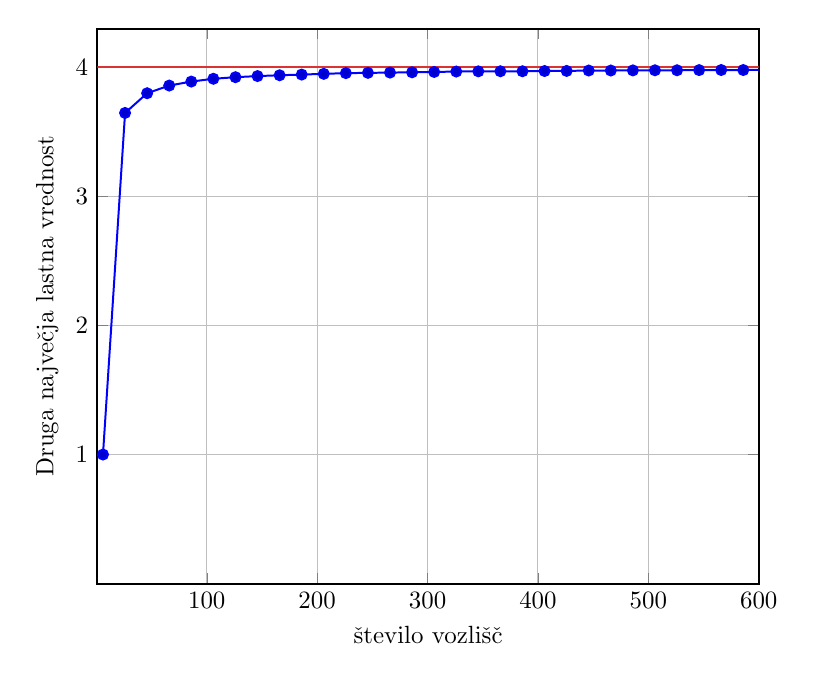
\begin{tikzpicture}[scale=0.9]
        \definecolor{pleasantred}{rgb}{0.85, 0.2, 0.2}
        \begin{axis}[
            xlabel={število vozlišč},
            width=0.9\textwidth,
            ylabel={Druga največja lastna vrednost},
            grid=major,
            ymin=0, ymax=4.3,
            xmin=1, xmax=600,
            xtick={0,100,...,600},
            ytick={1,2,3,4},
            thick
            ]
            \draw[draw=pleasantred] (axis cs:0,4) -- (axis cs:600,4);
            \addplot coordinates {
                (6, 1.0000000000000002)
                (26, 3.6469425449844923)
                (46, 3.79963239469457)
                (66, 3.8590979945057677)
                (86, 3.8900142704961667)
                (106, 3.9116565426594128)
                (126, 3.9238905598334965)
                (146, 3.9325600246589594)
                (166, 3.938855777384826)
                (186, 3.944147515902753)
                (206, 3.9498671033019517)
                (226, 3.9552616354117065)
                (246, 3.957467810537496)
                (266, 3.959490001307144)
                (286, 3.9618796798493063)
                (306, 3.9644616694659205)
                (326, 3.9676602186376644)
                (346, 3.9692542741810946)
                (366, 3.9698360851495904)
                (386, 3.9698257500021206)
                (406, 3.97181111813395)
                (426, 3.972473010011027)
                (446, 3.975603794486935)
                (466, 3.9756303352387716)
                (486, 3.9766439267420317)
                (506, 3.977488063510781)
                (526, 3.9776682760947293)
                (546, 3.978964750149576)
                (566, 3.979531750065059)
                (586, 3.9794685667065974)
                (606, 3.9811456508027763)
                };
            \end{axis}
        \end{tikzpicture}
        \caption{Graf povprečij \(\lambda(G)\) \(5\)-regularnih grafov v odvisnosti od števila vozlišč}
        \label{fig:5-regular}
\end{figure}

Na sliki \ref{fig:5-regular} vidimo, da se povprečje lastnih vrednosti približuje ravno meji za Ramanujanove grafe! Postopek ponovimo še za grafe s stopnjama \(d=11\) in \(d=21\) in tudi v teh primerih opazimo približevanje Ramanujanovi meji.
\begin{figure}[t]
    \centering
    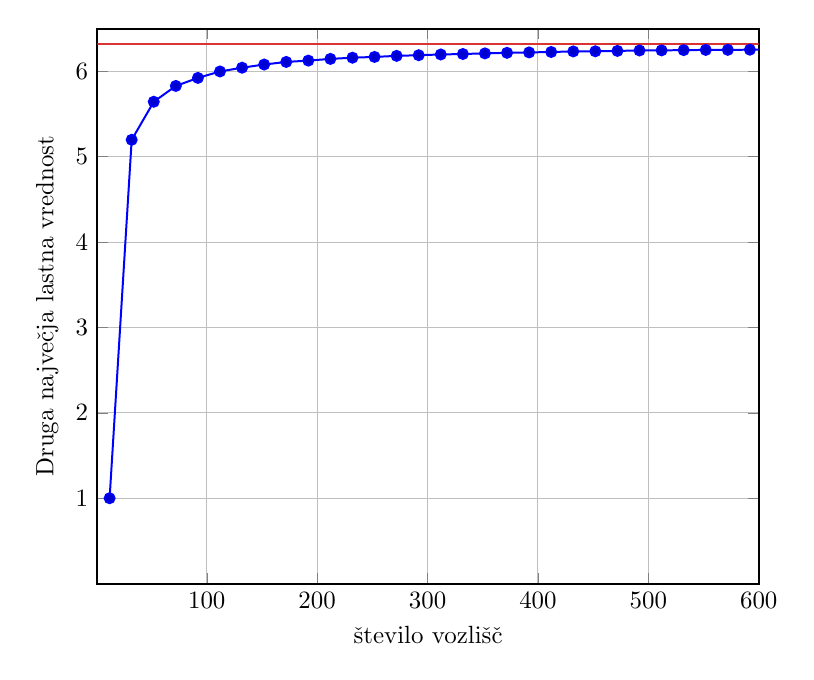
\begin{tikzpicture}[scale=0.9]
        \definecolor{pleasantred}{rgb}{0.85, 0.2, 0.2}
        \begin{axis}[
            xlabel={število vozlišč},
            width=0.9\textwidth,
            ylabel={Druga največja lastna vrednost},
                grid=major,
                ymin=0, ymax=6.5,
                xmin=1, xmax=600,
                xtick={0,100,...,600},
                ytick={1,2,3,4,5,6},
                thick
            ]
            \draw[draw=pleasantred] (axis cs:0,6.324555320336759) -- (axis cs:600,6.324555320336759);
            \addplot coordinates {
                (12, 1.0000000000000002)
                (32, 5.198156377614785)
                (52, 5.643885284747165)
                (72, 5.829117444893516)
                (92, 5.923172524513979)
                (112, 5.998622178810724)
                (132, 6.042619064245882)
                (152, 6.079957685856226)
                (172, 6.11026242602795)
                (192, 6.125752222542846)
                (212, 6.14580019144193)
                (232, 6.159810079904397)
                (252, 6.168875088596623)
                (272, 6.18128569012168)
                (292, 6.189017996514279)
                (312, 6.197667854719561)
                (332, 6.203055775141022)
                (352, 6.210376446059419)
                (372, 6.2170465023897865)
                (392, 6.221533675435159)
                (412, 6.226668634957975)
                (432, 6.23348367206533)
                (452, 6.234805834700305)
                (472, 6.23927709112199)
                (492, 6.244446713350618)
                (512, 6.24568687387802)
                (532, 6.248511105653832)
                (552, 6.25088144542781)
                (572, 6.251713414323658)
                (592, 6.253516933929778)
                (612, 6.254946081316828)
                };
        \end{axis}
    \end{tikzpicture}
    \caption{Graf povprečij \(\lambda(G)\) \(11\)-regularnih grafov v odvisnosti od števila vozlišč}
    \label{fig:11-regular}
\end{figure}

\begin{figure}[t]
    \centering
    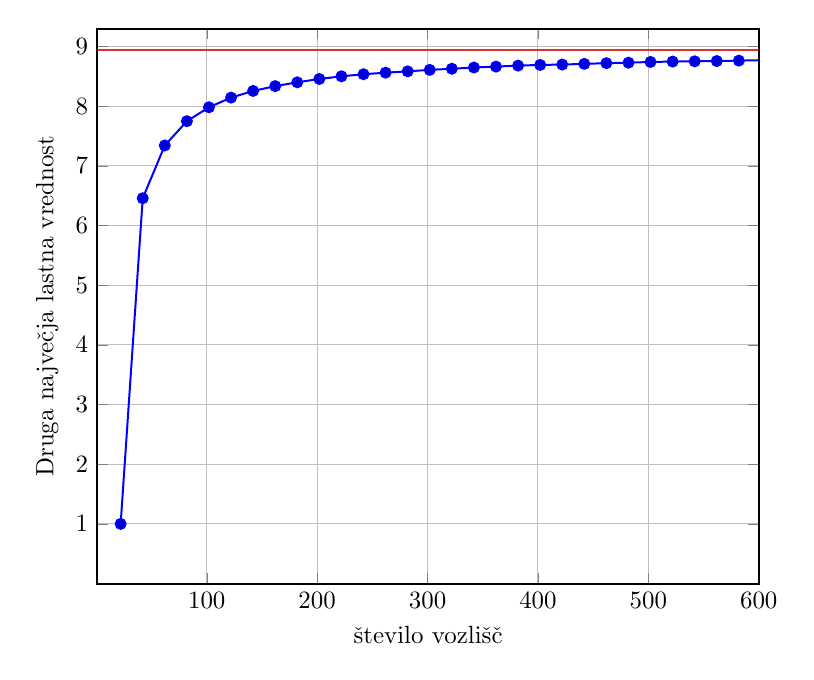
\begin{tikzpicture}[scale=0.9]
        \definecolor{pleasantred}{rgb}{0.85, 0.2, 0.2}
        \begin{axis}[
            xlabel={število vozlišč},
            width=0.9\textwidth,
            ylabel={Druga največja lastna vrednost},
            grid=major,
            ymin=0, ymax=9.3,
            xmin=1, xmax=600,
            xtick={0,100,...,600},
            ytick={1,2,3,4,5,6,7,8,9},
            thick
            ]
            \draw[draw=pleasantred] (axis cs:0,8.94427190999916) -- (axis cs:600,8.94427190999916);
            \addplot coordinates {
                (22, 1.0000000000000016)
                (42, 6.457762460689075)
                (62, 7.34267381875069)
                (82, 7.749182706134452)
                (102, 7.9826028554188175)
                (122, 8.144251955483162)
                (142, 8.256172883115111)
                (162, 8.33681314660636)
                (182, 8.400759701073772)
                (202, 8.456929688398343)
                (222, 8.50117677868208)
                (242, 8.536147098061887)
                (262, 8.562439059545776)
                (282, 8.584384770184979)
                (302, 8.609496150772358)
                (322, 8.627941976386401)
                (342, 8.649075592875864)
                (362, 8.664258721715953)
                (382, 8.680621349648668)
                (402, 8.691973426726586)
                (422, 8.69812122565171)
                (442, 8.709986877027816)
                (462, 8.72164670988282)
                (482, 8.729634460708713)
                (502, 8.741916828498463)
                (522, 8.748384221744477)
                (542, 8.75275208966012)
                (562, 8.757330480876565)
                (582, 8.764164575308484)
                (602, 8.771656193932213)
                };
            \end{axis}
        \end{tikzpicture}
        \caption{Graf povprečij \(\lambda(G)\) \(21\)-regularnih grafov v odvisnosti od števila vozlišč}
        \label{fig:21-regular}
    \end{figure}

\subsection{Delež Ramanujanovih grafov}
Nadaljujemo z deležom Ramanujanovih grafov. Postopek bo enak kot prej, le da rišemo vse hkrati na enem grafu. Da dobimo boljše rezultate si tokrat ogledamo tudi grafe z več vozlišči. Začnemo z grafi, ki imajo manj kot \(1000\) vozlišč, za tem pa tudi izračunamo delež Ramanujanovih grafov za grafe z do \(10^5\) vozlišči. Zaradi časovne zahtevnosti za tako velike grafe izračunamo delež v korakih po \(10 000\) vozlišč. Pri tako velikih grafih je za sosednostne matrike potrebno uporabljati razpršene matrike, da prostorska zahtevnost raste linearno in ne kvadratično. Brez razpršenih matrik bi v primeru \(n=10^5\) in \(d=21\) program porabil okoli \(40\) GB pomnilnika, če pa uporabimo razpršene matrike pa le okoli \(10\) MB.

\begin{figure}[t]
    \centering
    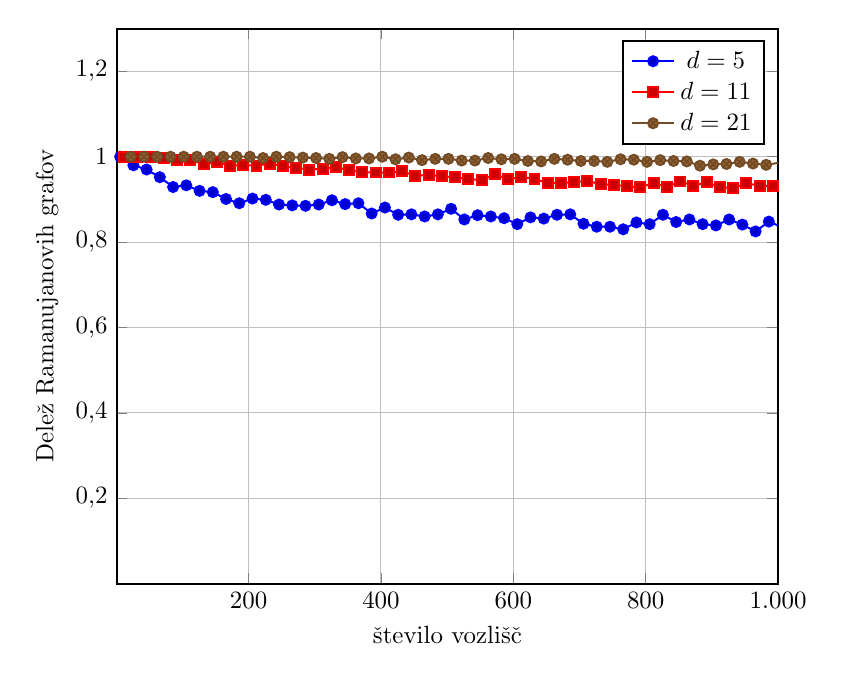
\begin{tikzpicture}[scale=0.9]
        \begin{axis}[
                xlabel={število vozlišč},
                width=0.9\textwidth,
                ylabel={Delež Ramanujanovih grafov},
                grid=major,
                ymin=0, ymax=1.3,
                xmin=1, xmax=1000,
                xtick={0,200,...,1000},
                ytick={0.2,0.4,0.6,0.8,1,1.2},
                tick label style={/pgf/number format/use comma},
                thick
            ]
            \addplot coordinates {
                (6, 1.0)
                (26, 0.98)
                (46, 0.97)
                (66, 0.952)
                (86, 0.929)
                (106, 0.933)
                (126, 0.92)
                (146, 0.917)
                (166, 0.901)
                (186, 0.891)
                (206, 0.902)
                (226, 0.899)
                (246, 0.888)
                (266, 0.886)
                (286, 0.885)
                (306, 0.888)
                (326, 0.898)
                (346, 0.889)
                (366, 0.891)
                (386, 0.867)
                (406, 0.881)
                (426, 0.864)
                (446, 0.865)
                (466, 0.86)
                (486, 0.865)
                (506, 0.878)
                (526, 0.853)
                (546, 0.863)
                (566, 0.86)
                (586, 0.856)
                (606, 0.842)
                (626, 0.858)
                (646, 0.855)
                (666, 0.864)
                (686, 0.865)
                (706, 0.843)
                (726, 0.836)
                (746, 0.836)
                (766, 0.83)
                (786, 0.846)
                (806, 0.842)
                (826, 0.864)
                (846, 0.847)
                (866, 0.853)
                (886, 0.842)
                (906, 0.839)
                (926, 0.853)
                (946, 0.841)
                (966, 0.825)
                (986, 0.848)
                (1006, 0.835)
                };
            \addlegendentry{\(d=5\)}
            \addplot coordinates {
                (12, 1.0)
                (32, 1.0)
                (52, 0.999)
                (72, 0.996)
                (92, 0.993)
                (112, 0.992)
                (132, 0.983)
                (152, 0.987)
                (172, 0.979)
                (192, 0.98)
                (212, 0.979)
                (232, 0.984)
                (252, 0.978)
                (272, 0.974)
                (292, 0.97)
                (312, 0.972)
                (332, 0.976)
                (352, 0.968)
                (372, 0.964)
                (392, 0.963)
                (412, 0.963)
                (432, 0.966)
                (452, 0.955)
                (472, 0.958)
                (492, 0.954)
                (512, 0.952)
                (532, 0.948)
                (552, 0.945)
                (572, 0.959)
                (592, 0.947)
                (612, 0.953)
                (632, 0.948)
                (652, 0.938)
                (672, 0.939)
                (692, 0.94)
                (712, 0.944)
                (732, 0.935)
                (752, 0.934)
                (772, 0.931)
                (792, 0.928)
                (812, 0.939)
                (832, 0.929)
                (852, 0.942)
                (872, 0.932)
                (892, 0.94)
                (912, 0.929)
                (932, 0.926)
                (952, 0.938)
                (972, 0.932)
                (992, 0.931)
                (1012, 0.923)
                };
                \addlegendentry{\(d=11\)}
                \addplot coordinates {
                    (22, 1.0)
                    (42, 1.0)
                    (62, 1.0)
                    (82, 1.0)
                    (102, 1.0)
                    (122, 1.0)
                    (142, 1.0)
                    (162, 1.0)
                    (182, 1.0)
                    (202, 1.0)
                    (222, 0.997)
                    (242, 1.0)
                    (262, 0.999)
                    (282, 0.998)
                    (302, 0.997)
                    (322, 0.995)
                    (342, 0.999)
                    (362, 0.996)
                    (382, 0.996)
                    (402, 1.0)
                    (422, 0.994)
                    (442, 0.998)
                    (462, 0.992)
                    (482, 0.995)
                    (502, 0.995)
                    (522, 0.991)
                    (542, 0.991)
                    (562, 0.997)
                    (582, 0.994)
                    (602, 0.995)
                    (622, 0.99)
                    (642, 0.989)
                    (662, 0.995)
                    (682, 0.993)
                    (702, 0.99)
                    (722, 0.99)
                    (742, 0.988)
                    (762, 0.994)
                    (782, 0.993)
                    (802, 0.988)
                    (822, 0.992)
                    (842, 0.99)
                    (862, 0.989)
                    (882, 0.979)
                    (902, 0.982)
                    (922, 0.983)
                    (942, 0.988)
                    (962, 0.984)
                    (982, 0.981)
                    (1002, 0.986)
                    };
                    \addlegendentry{\(d=21\)}   
        \end{axis}
    \end{tikzpicture}
    \caption{Graf deleža Ramanujanovih grafov od 1 do 300}
\end{figure}
\begin{figure}[H]
    \centering
    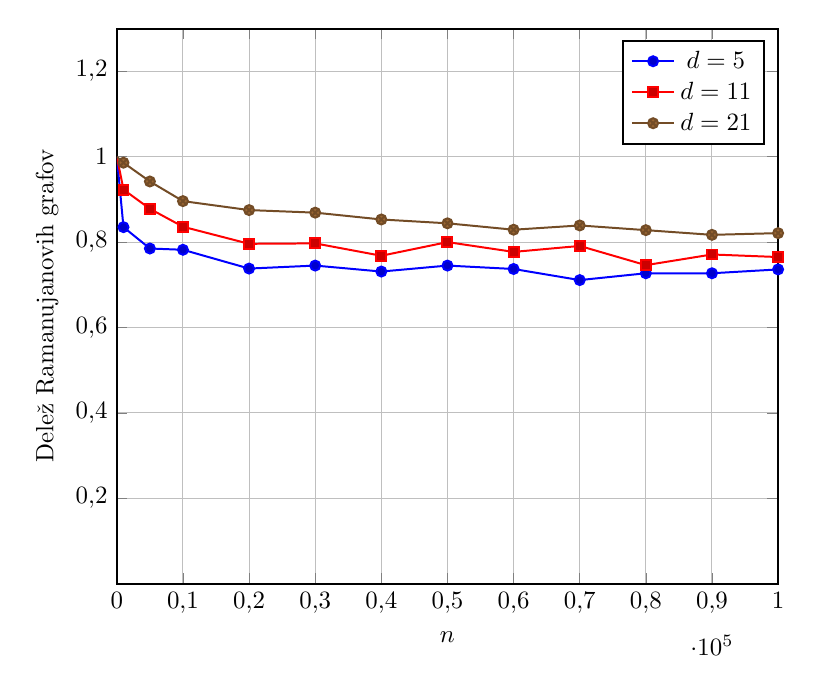
\begin{tikzpicture}[scale=0.9]
        \begin{axis}[
                xlabel={$n$},
                width=0.9\textwidth,
                ylabel={Delež Ramanujanovih grafov},
                grid=major,
                ymin=0, ymax=1.3,
                xmin=1, xmax=100000,
                xtick={0,10000,...,100000},
                ytick={0.2,0.4,0.6,0.8,1,1.2},
                tick label style={/pgf/number format/use comma},
                thick
            ]
            \addplot coordinates {
                (0, 1.0)
                (1006, 0.835)
                (5000, 0.785)
                (10000, 0.782)
                (20000, 0.738)
                (30000, 0.745)
                (40000, 0.731)
                (50000, 0.745)
                (60000, 0.737)
                (70000, 0.711)
                (80000, 0.727)
                (90000, 0.727)
                (100000, 0.736)
                };
                \addlegendentry{\(d=5\)}
            \addplot coordinates {
                (0, 1.0)
                (1012, 0.923)
                (5000, 0.878)
                (10000, 0.836)
                (20000, 0.796)
                (30000, 0.797)
                (40000, 0.768)
                (50000, 0.8)
                (60000, 0.777)
                (70000, 0.791)
                (80000, 0.746)
                (90000, 0.771)
                (100000, 0.765)
                };
                \addlegendentry{\(d=11\)}
            \addplot coordinates {
                (0, 1.0)
                (1002, 0.986)
                (5000, 0.942)
                (10000, 0.896)
                (20000, 0.875)
                (30000, 0.869)
                (40000, 0.853)
                (50000, 0.844)
                (60000, 0.829)
                (70000, 0.839)
                (80000, 0.828)
                (90000, 0.817)
                (100000, 0.821)
                };
                \addlegendentry{\(d=21\)}
    \end{axis}
    \end{tikzpicture}
    \caption{Graf deleža Ramanujanovih grafov od 10000 do 100000}
\end{figure}
Na grafih vidimo, da se delež Ramanujanovih grafov z večanjem števila vozlišč zmanjšuje. Vidimo pa tudi, da se ta delež zmanjšuje hitreje pri nižjih stopnjah regularnosti. Najpomembnejše pa je, da se ta delež ne približuje \(0\), ne glede na stopnjo regularnosti; na grafih vidimo, da se delež približuje približno \(70\%\), vendar je težko trditi, saj kljub velikemu številu vozlišč še vedno ni vidne končne konvergence. Dokaza za to trditev si ne bomo ogledali, je bilo pa nedavno dokazano, da je delež Ramanujanovih grafov asimptotično neodvisen od stopnje regularnosti in se približuje približno \(69\%\) \cite{huang2024ramanujanpropertyedgeuniversality}. Ključni del dokaza je bil, da so izračunali, da se porazdelitev največje netrivialne lastne vrednosti približuje Tracy-Widomovi porazdelitvi. Za to porazdelitev pa lahko preverimo, kolikšno maso ima pod Ramanujanovo mejo. Omenjeni članek predstavlja pomemben preboj v teoriji Ramanujanovih grafov, saj je bila porazdelitev lastnih vrednosti, prav tako pa delež Ramanujanovih grafov, dolgo obstoječ odprt problem.

\begin{figure}[H]
    \begin{center}
        %% Creator: Matplotlib, PGF backend
%%
%% To include the figure in your LaTeX document, write
%%   \input{<filename>.pgf}
%%
%% Make sure the required packages are loaded in your preamble
%%   \usepackage{pgf}
%%
%% Also ensure that all the required font packages are loaded; for instance,
%% the lmodern package is sometimes necessary when using math font.
%%   \usepackage{lmodern}
%%
%% Figures using additional raster images can only be included by \input if
%% they are in the same directory as the main LaTeX file. For loading figures
%% from other directories you can use the `import` package
%%   \usepackage{import}
%%
%% and then include the figures with
%%   \import{<path to file>}{<filename>.pgf}
%%
%% Matplotlib used the following preamble
%%   \def\mathdefault#1{#1}
%%   \everymath=\expandafter{\the\everymath\displaystyle}
%%   \IfFileExists{scrextend.sty}{
%%     \usepackage[fontsize=10.000000pt]{scrextend}
%%   }{
%%     \renewcommand{\normalsize}{\fontsize{10.000000}{12.000000}\selectfont}
%%     \normalsize
%%   }
%%   
%%   \makeatletter\@ifpackageloaded{underscore}{}{\usepackage[strings]{underscore}}\makeatother
%%
\begingroup%
\makeatletter%
\begin{pgfpicture}%
\pgfpathrectangle{\pgfpointorigin}{\pgfqpoint{5.906660in}{6.000000in}}%
\pgfusepath{use as bounding box, clip}%
\begin{pgfscope}%
\pgfsetbuttcap%
\pgfsetmiterjoin%
\definecolor{currentfill}{rgb}{1.000000,1.000000,1.000000}%
\pgfsetfillcolor{currentfill}%
\pgfsetlinewidth{0.000000pt}%
\definecolor{currentstroke}{rgb}{1.000000,1.000000,1.000000}%
\pgfsetstrokecolor{currentstroke}%
\pgfsetdash{}{0pt}%
\pgfpathmoveto{\pgfqpoint{0.000000in}{0.000000in}}%
\pgfpathlineto{\pgfqpoint{5.906660in}{0.000000in}}%
\pgfpathlineto{\pgfqpoint{5.906660in}{6.000000in}}%
\pgfpathlineto{\pgfqpoint{0.000000in}{6.000000in}}%
\pgfpathlineto{\pgfqpoint{0.000000in}{0.000000in}}%
\pgfpathclose%
\pgfusepath{fill}%
\end{pgfscope}%
\begin{pgfscope}%
\pgfsetbuttcap%
\pgfsetmiterjoin%
\definecolor{currentfill}{rgb}{1.000000,1.000000,1.000000}%
\pgfsetfillcolor{currentfill}%
\pgfsetlinewidth{0.000000pt}%
\definecolor{currentstroke}{rgb}{0.000000,0.000000,0.000000}%
\pgfsetstrokecolor{currentstroke}%
\pgfsetstrokeopacity{0.000000}%
\pgfsetdash{}{0pt}%
\pgfpathmoveto{\pgfqpoint{0.819028in}{0.582778in}}%
\pgfpathlineto{\pgfqpoint{5.756660in}{0.582778in}}%
\pgfpathlineto{\pgfqpoint{5.756660in}{5.850000in}}%
\pgfpathlineto{\pgfqpoint{0.819028in}{5.850000in}}%
\pgfpathlineto{\pgfqpoint{0.819028in}{0.582778in}}%
\pgfpathclose%
\pgfusepath{fill}%
\end{pgfscope}%
\begin{pgfscope}%
\pgfpathrectangle{\pgfqpoint{0.819028in}{0.582778in}}{\pgfqpoint{4.937632in}{5.267222in}}%
\pgfusepath{clip}%
\pgfsetbuttcap%
\pgfsetmiterjoin%
\definecolor{currentfill}{rgb}{0.121569,0.466667,0.705882}%
\pgfsetfillcolor{currentfill}%
\pgfsetfillopacity{0.700000}%
\pgfsetlinewidth{1.003750pt}%
\definecolor{currentstroke}{rgb}{0.000000,0.000000,0.000000}%
\pgfsetstrokecolor{currentstroke}%
\pgfsetstrokeopacity{0.700000}%
\pgfsetdash{}{0pt}%
\pgfpathmoveto{\pgfqpoint{1.043466in}{0.582778in}}%
\pgfpathlineto{\pgfqpoint{1.193091in}{0.582778in}}%
\pgfpathlineto{\pgfqpoint{1.193091in}{0.605253in}}%
\pgfpathlineto{\pgfqpoint{1.043466in}{0.605253in}}%
\pgfpathlineto{\pgfqpoint{1.043466in}{0.582778in}}%
\pgfpathclose%
\pgfusepath{stroke,fill}%
\end{pgfscope}%
\begin{pgfscope}%
\pgfpathrectangle{\pgfqpoint{0.819028in}{0.582778in}}{\pgfqpoint{4.937632in}{5.267222in}}%
\pgfusepath{clip}%
\pgfsetbuttcap%
\pgfsetmiterjoin%
\definecolor{currentfill}{rgb}{0.121569,0.466667,0.705882}%
\pgfsetfillcolor{currentfill}%
\pgfsetfillopacity{0.700000}%
\pgfsetlinewidth{1.003750pt}%
\definecolor{currentstroke}{rgb}{0.000000,0.000000,0.000000}%
\pgfsetstrokecolor{currentstroke}%
\pgfsetstrokeopacity{0.700000}%
\pgfsetdash{}{0pt}%
\pgfpathmoveto{\pgfqpoint{1.193091in}{0.582778in}}%
\pgfpathlineto{\pgfqpoint{1.342716in}{0.582778in}}%
\pgfpathlineto{\pgfqpoint{1.342716in}{0.650203in}}%
\pgfpathlineto{\pgfqpoint{1.193091in}{0.650203in}}%
\pgfpathlineto{\pgfqpoint{1.193091in}{0.582778in}}%
\pgfpathclose%
\pgfusepath{stroke,fill}%
\end{pgfscope}%
\begin{pgfscope}%
\pgfpathrectangle{\pgfqpoint{0.819028in}{0.582778in}}{\pgfqpoint{4.937632in}{5.267222in}}%
\pgfusepath{clip}%
\pgfsetbuttcap%
\pgfsetmiterjoin%
\definecolor{currentfill}{rgb}{0.121569,0.466667,0.705882}%
\pgfsetfillcolor{currentfill}%
\pgfsetfillopacity{0.700000}%
\pgfsetlinewidth{1.003750pt}%
\definecolor{currentstroke}{rgb}{0.000000,0.000000,0.000000}%
\pgfsetstrokecolor{currentstroke}%
\pgfsetstrokeopacity{0.700000}%
\pgfsetdash{}{0pt}%
\pgfpathmoveto{\pgfqpoint{1.342716in}{0.582778in}}%
\pgfpathlineto{\pgfqpoint{1.492341in}{0.582778in}}%
\pgfpathlineto{\pgfqpoint{1.492341in}{0.758082in}}%
\pgfpathlineto{\pgfqpoint{1.342716in}{0.758082in}}%
\pgfpathlineto{\pgfqpoint{1.342716in}{0.582778in}}%
\pgfpathclose%
\pgfusepath{stroke,fill}%
\end{pgfscope}%
\begin{pgfscope}%
\pgfpathrectangle{\pgfqpoint{0.819028in}{0.582778in}}{\pgfqpoint{4.937632in}{5.267222in}}%
\pgfusepath{clip}%
\pgfsetbuttcap%
\pgfsetmiterjoin%
\definecolor{currentfill}{rgb}{0.121569,0.466667,0.705882}%
\pgfsetfillcolor{currentfill}%
\pgfsetfillopacity{0.700000}%
\pgfsetlinewidth{1.003750pt}%
\definecolor{currentstroke}{rgb}{0.000000,0.000000,0.000000}%
\pgfsetstrokecolor{currentstroke}%
\pgfsetstrokeopacity{0.700000}%
\pgfsetdash{}{0pt}%
\pgfpathmoveto{\pgfqpoint{1.492341in}{0.582778in}}%
\pgfpathlineto{\pgfqpoint{1.641966in}{0.582778in}}%
\pgfpathlineto{\pgfqpoint{1.641966in}{1.077226in}}%
\pgfpathlineto{\pgfqpoint{1.492341in}{1.077226in}}%
\pgfpathlineto{\pgfqpoint{1.492341in}{0.582778in}}%
\pgfpathclose%
\pgfusepath{stroke,fill}%
\end{pgfscope}%
\begin{pgfscope}%
\pgfpathrectangle{\pgfqpoint{0.819028in}{0.582778in}}{\pgfqpoint{4.937632in}{5.267222in}}%
\pgfusepath{clip}%
\pgfsetbuttcap%
\pgfsetmiterjoin%
\definecolor{currentfill}{rgb}{0.121569,0.466667,0.705882}%
\pgfsetfillcolor{currentfill}%
\pgfsetfillopacity{0.700000}%
\pgfsetlinewidth{1.003750pt}%
\definecolor{currentstroke}{rgb}{0.000000,0.000000,0.000000}%
\pgfsetstrokecolor{currentstroke}%
\pgfsetstrokeopacity{0.700000}%
\pgfsetdash{}{0pt}%
\pgfpathmoveto{\pgfqpoint{1.641966in}{0.582778in}}%
\pgfpathlineto{\pgfqpoint{1.791592in}{0.582778in}}%
\pgfpathlineto{\pgfqpoint{1.791592in}{1.670564in}}%
\pgfpathlineto{\pgfqpoint{1.641966in}{1.670564in}}%
\pgfpathlineto{\pgfqpoint{1.641966in}{0.582778in}}%
\pgfpathclose%
\pgfusepath{stroke,fill}%
\end{pgfscope}%
\begin{pgfscope}%
\pgfpathrectangle{\pgfqpoint{0.819028in}{0.582778in}}{\pgfqpoint{4.937632in}{5.267222in}}%
\pgfusepath{clip}%
\pgfsetbuttcap%
\pgfsetmiterjoin%
\definecolor{currentfill}{rgb}{0.121569,0.466667,0.705882}%
\pgfsetfillcolor{currentfill}%
\pgfsetfillopacity{0.700000}%
\pgfsetlinewidth{1.003750pt}%
\definecolor{currentstroke}{rgb}{0.000000,0.000000,0.000000}%
\pgfsetstrokecolor{currentstroke}%
\pgfsetstrokeopacity{0.700000}%
\pgfsetdash{}{0pt}%
\pgfpathmoveto{\pgfqpoint{1.791592in}{0.582778in}}%
\pgfpathlineto{\pgfqpoint{1.941217in}{0.582778in}}%
\pgfpathlineto{\pgfqpoint{1.941217in}{2.227942in}}%
\pgfpathlineto{\pgfqpoint{1.791592in}{2.227942in}}%
\pgfpathlineto{\pgfqpoint{1.791592in}{0.582778in}}%
\pgfpathclose%
\pgfusepath{stroke,fill}%
\end{pgfscope}%
\begin{pgfscope}%
\pgfpathrectangle{\pgfqpoint{0.819028in}{0.582778in}}{\pgfqpoint{4.937632in}{5.267222in}}%
\pgfusepath{clip}%
\pgfsetbuttcap%
\pgfsetmiterjoin%
\definecolor{currentfill}{rgb}{0.121569,0.466667,0.705882}%
\pgfsetfillcolor{currentfill}%
\pgfsetfillopacity{0.700000}%
\pgfsetlinewidth{1.003750pt}%
\definecolor{currentstroke}{rgb}{0.000000,0.000000,0.000000}%
\pgfsetstrokecolor{currentstroke}%
\pgfsetstrokeopacity{0.700000}%
\pgfsetdash{}{0pt}%
\pgfpathmoveto{\pgfqpoint{1.941217in}{0.582778in}}%
\pgfpathlineto{\pgfqpoint{2.090842in}{0.582778in}}%
\pgfpathlineto{\pgfqpoint{2.090842in}{3.167394in}}%
\pgfpathlineto{\pgfqpoint{1.941217in}{3.167394in}}%
\pgfpathlineto{\pgfqpoint{1.941217in}{0.582778in}}%
\pgfpathclose%
\pgfusepath{stroke,fill}%
\end{pgfscope}%
\begin{pgfscope}%
\pgfpathrectangle{\pgfqpoint{0.819028in}{0.582778in}}{\pgfqpoint{4.937632in}{5.267222in}}%
\pgfusepath{clip}%
\pgfsetbuttcap%
\pgfsetmiterjoin%
\definecolor{currentfill}{rgb}{0.121569,0.466667,0.705882}%
\pgfsetfillcolor{currentfill}%
\pgfsetfillopacity{0.700000}%
\pgfsetlinewidth{1.003750pt}%
\definecolor{currentstroke}{rgb}{0.000000,0.000000,0.000000}%
\pgfsetstrokecolor{currentstroke}%
\pgfsetstrokeopacity{0.700000}%
\pgfsetdash{}{0pt}%
\pgfpathmoveto{\pgfqpoint{2.090842in}{0.582778in}}%
\pgfpathlineto{\pgfqpoint{2.240467in}{0.582778in}}%
\pgfpathlineto{\pgfqpoint{2.240467in}{3.864116in}}%
\pgfpathlineto{\pgfqpoint{2.090842in}{3.864116in}}%
\pgfpathlineto{\pgfqpoint{2.090842in}{0.582778in}}%
\pgfpathclose%
\pgfusepath{stroke,fill}%
\end{pgfscope}%
\begin{pgfscope}%
\pgfpathrectangle{\pgfqpoint{0.819028in}{0.582778in}}{\pgfqpoint{4.937632in}{5.267222in}}%
\pgfusepath{clip}%
\pgfsetbuttcap%
\pgfsetmiterjoin%
\definecolor{currentfill}{rgb}{0.121569,0.466667,0.705882}%
\pgfsetfillcolor{currentfill}%
\pgfsetfillopacity{0.700000}%
\pgfsetlinewidth{1.003750pt}%
\definecolor{currentstroke}{rgb}{0.000000,0.000000,0.000000}%
\pgfsetstrokecolor{currentstroke}%
\pgfsetstrokeopacity{0.700000}%
\pgfsetdash{}{0pt}%
\pgfpathmoveto{\pgfqpoint{2.240467in}{0.582778in}}%
\pgfpathlineto{\pgfqpoint{2.390093in}{0.582778in}}%
\pgfpathlineto{\pgfqpoint{2.390093in}{4.763113in}}%
\pgfpathlineto{\pgfqpoint{2.240467in}{4.763113in}}%
\pgfpathlineto{\pgfqpoint{2.240467in}{0.582778in}}%
\pgfpathclose%
\pgfusepath{stroke,fill}%
\end{pgfscope}%
\begin{pgfscope}%
\pgfpathrectangle{\pgfqpoint{0.819028in}{0.582778in}}{\pgfqpoint{4.937632in}{5.267222in}}%
\pgfusepath{clip}%
\pgfsetbuttcap%
\pgfsetmiterjoin%
\definecolor{currentfill}{rgb}{0.121569,0.466667,0.705882}%
\pgfsetfillcolor{currentfill}%
\pgfsetfillopacity{0.700000}%
\pgfsetlinewidth{1.003750pt}%
\definecolor{currentstroke}{rgb}{0.000000,0.000000,0.000000}%
\pgfsetstrokecolor{currentstroke}%
\pgfsetstrokeopacity{0.700000}%
\pgfsetdash{}{0pt}%
\pgfpathmoveto{\pgfqpoint{2.390093in}{0.582778in}}%
\pgfpathlineto{\pgfqpoint{2.539718in}{0.582778in}}%
\pgfpathlineto{\pgfqpoint{2.539718in}{4.830538in}}%
\pgfpathlineto{\pgfqpoint{2.390093in}{4.830538in}}%
\pgfpathlineto{\pgfqpoint{2.390093in}{0.582778in}}%
\pgfpathclose%
\pgfusepath{stroke,fill}%
\end{pgfscope}%
\begin{pgfscope}%
\pgfpathrectangle{\pgfqpoint{0.819028in}{0.582778in}}{\pgfqpoint{4.937632in}{5.267222in}}%
\pgfusepath{clip}%
\pgfsetbuttcap%
\pgfsetmiterjoin%
\definecolor{currentfill}{rgb}{0.121569,0.466667,0.705882}%
\pgfsetfillcolor{currentfill}%
\pgfsetfillopacity{0.700000}%
\pgfsetlinewidth{1.003750pt}%
\definecolor{currentstroke}{rgb}{0.000000,0.000000,0.000000}%
\pgfsetstrokecolor{currentstroke}%
\pgfsetstrokeopacity{0.700000}%
\pgfsetdash{}{0pt}%
\pgfpathmoveto{\pgfqpoint{2.539718in}{0.582778in}}%
\pgfpathlineto{\pgfqpoint{2.689343in}{0.582778in}}%
\pgfpathlineto{\pgfqpoint{2.689343in}{5.599180in}}%
\pgfpathlineto{\pgfqpoint{2.539718in}{5.599180in}}%
\pgfpathlineto{\pgfqpoint{2.539718in}{0.582778in}}%
\pgfpathclose%
\pgfusepath{stroke,fill}%
\end{pgfscope}%
\begin{pgfscope}%
\pgfpathrectangle{\pgfqpoint{0.819028in}{0.582778in}}{\pgfqpoint{4.937632in}{5.267222in}}%
\pgfusepath{clip}%
\pgfsetbuttcap%
\pgfsetmiterjoin%
\definecolor{currentfill}{rgb}{0.121569,0.466667,0.705882}%
\pgfsetfillcolor{currentfill}%
\pgfsetfillopacity{0.700000}%
\pgfsetlinewidth{1.003750pt}%
\definecolor{currentstroke}{rgb}{0.000000,0.000000,0.000000}%
\pgfsetstrokecolor{currentstroke}%
\pgfsetstrokeopacity{0.700000}%
\pgfsetdash{}{0pt}%
\pgfpathmoveto{\pgfqpoint{2.689343in}{0.582778in}}%
\pgfpathlineto{\pgfqpoint{2.838968in}{0.582778in}}%
\pgfpathlineto{\pgfqpoint{2.838968in}{5.369936in}}%
\pgfpathlineto{\pgfqpoint{2.689343in}{5.369936in}}%
\pgfpathlineto{\pgfqpoint{2.689343in}{0.582778in}}%
\pgfpathclose%
\pgfusepath{stroke,fill}%
\end{pgfscope}%
\begin{pgfscope}%
\pgfpathrectangle{\pgfqpoint{0.819028in}{0.582778in}}{\pgfqpoint{4.937632in}{5.267222in}}%
\pgfusepath{clip}%
\pgfsetbuttcap%
\pgfsetmiterjoin%
\definecolor{currentfill}{rgb}{0.121569,0.466667,0.705882}%
\pgfsetfillcolor{currentfill}%
\pgfsetfillopacity{0.700000}%
\pgfsetlinewidth{1.003750pt}%
\definecolor{currentstroke}{rgb}{0.000000,0.000000,0.000000}%
\pgfsetstrokecolor{currentstroke}%
\pgfsetstrokeopacity{0.700000}%
\pgfsetdash{}{0pt}%
\pgfpathmoveto{\pgfqpoint{2.838968in}{0.582778in}}%
\pgfpathlineto{\pgfqpoint{2.988593in}{0.582778in}}%
\pgfpathlineto{\pgfqpoint{2.988593in}{4.965387in}}%
\pgfpathlineto{\pgfqpoint{2.838968in}{4.965387in}}%
\pgfpathlineto{\pgfqpoint{2.838968in}{0.582778in}}%
\pgfpathclose%
\pgfusepath{stroke,fill}%
\end{pgfscope}%
\begin{pgfscope}%
\pgfpathrectangle{\pgfqpoint{0.819028in}{0.582778in}}{\pgfqpoint{4.937632in}{5.267222in}}%
\pgfusepath{clip}%
\pgfsetbuttcap%
\pgfsetmiterjoin%
\definecolor{currentfill}{rgb}{0.121569,0.466667,0.705882}%
\pgfsetfillcolor{currentfill}%
\pgfsetfillopacity{0.700000}%
\pgfsetlinewidth{1.003750pt}%
\definecolor{currentstroke}{rgb}{0.000000,0.000000,0.000000}%
\pgfsetstrokecolor{currentstroke}%
\pgfsetstrokeopacity{0.700000}%
\pgfsetdash{}{0pt}%
\pgfpathmoveto{\pgfqpoint{2.988593in}{0.582778in}}%
\pgfpathlineto{\pgfqpoint{3.138219in}{0.582778in}}%
\pgfpathlineto{\pgfqpoint{3.138219in}{4.097855in}}%
\pgfpathlineto{\pgfqpoint{2.988593in}{4.097855in}}%
\pgfpathlineto{\pgfqpoint{2.988593in}{0.582778in}}%
\pgfpathclose%
\pgfusepath{stroke,fill}%
\end{pgfscope}%
\begin{pgfscope}%
\pgfpathrectangle{\pgfqpoint{0.819028in}{0.582778in}}{\pgfqpoint{4.937632in}{5.267222in}}%
\pgfusepath{clip}%
\pgfsetbuttcap%
\pgfsetmiterjoin%
\definecolor{currentfill}{rgb}{0.121569,0.466667,0.705882}%
\pgfsetfillcolor{currentfill}%
\pgfsetfillopacity{0.700000}%
\pgfsetlinewidth{1.003750pt}%
\definecolor{currentstroke}{rgb}{0.000000,0.000000,0.000000}%
\pgfsetstrokecolor{currentstroke}%
\pgfsetstrokeopacity{0.700000}%
\pgfsetdash{}{0pt}%
\pgfpathmoveto{\pgfqpoint{3.138219in}{0.582778in}}%
\pgfpathlineto{\pgfqpoint{3.287844in}{0.582778in}}%
\pgfpathlineto{\pgfqpoint{3.287844in}{3.419113in}}%
\pgfpathlineto{\pgfqpoint{3.138219in}{3.419113in}}%
\pgfpathlineto{\pgfqpoint{3.138219in}{0.582778in}}%
\pgfpathclose%
\pgfusepath{stroke,fill}%
\end{pgfscope}%
\begin{pgfscope}%
\pgfpathrectangle{\pgfqpoint{0.819028in}{0.582778in}}{\pgfqpoint{4.937632in}{5.267222in}}%
\pgfusepath{clip}%
\pgfsetbuttcap%
\pgfsetmiterjoin%
\definecolor{currentfill}{rgb}{0.121569,0.466667,0.705882}%
\pgfsetfillcolor{currentfill}%
\pgfsetfillopacity{0.700000}%
\pgfsetlinewidth{1.003750pt}%
\definecolor{currentstroke}{rgb}{0.000000,0.000000,0.000000}%
\pgfsetstrokecolor{currentstroke}%
\pgfsetstrokeopacity{0.700000}%
\pgfsetdash{}{0pt}%
\pgfpathmoveto{\pgfqpoint{3.287844in}{0.582778in}}%
\pgfpathlineto{\pgfqpoint{3.437469in}{0.582778in}}%
\pgfpathlineto{\pgfqpoint{3.437469in}{2.619006in}}%
\pgfpathlineto{\pgfqpoint{3.287844in}{2.619006in}}%
\pgfpathlineto{\pgfqpoint{3.287844in}{0.582778in}}%
\pgfpathclose%
\pgfusepath{stroke,fill}%
\end{pgfscope}%
\begin{pgfscope}%
\pgfpathrectangle{\pgfqpoint{0.819028in}{0.582778in}}{\pgfqpoint{4.937632in}{5.267222in}}%
\pgfusepath{clip}%
\pgfsetbuttcap%
\pgfsetmiterjoin%
\definecolor{currentfill}{rgb}{0.121569,0.466667,0.705882}%
\pgfsetfillcolor{currentfill}%
\pgfsetfillopacity{0.700000}%
\pgfsetlinewidth{1.003750pt}%
\definecolor{currentstroke}{rgb}{0.000000,0.000000,0.000000}%
\pgfsetstrokecolor{currentstroke}%
\pgfsetstrokeopacity{0.700000}%
\pgfsetdash{}{0pt}%
\pgfpathmoveto{\pgfqpoint{3.437469in}{0.582778in}}%
\pgfpathlineto{\pgfqpoint{3.587094in}{0.582778in}}%
\pgfpathlineto{\pgfqpoint{3.587094in}{2.138042in}}%
\pgfpathlineto{\pgfqpoint{3.437469in}{2.138042in}}%
\pgfpathlineto{\pgfqpoint{3.437469in}{0.582778in}}%
\pgfpathclose%
\pgfusepath{stroke,fill}%
\end{pgfscope}%
\begin{pgfscope}%
\pgfpathrectangle{\pgfqpoint{0.819028in}{0.582778in}}{\pgfqpoint{4.937632in}{5.267222in}}%
\pgfusepath{clip}%
\pgfsetbuttcap%
\pgfsetmiterjoin%
\definecolor{currentfill}{rgb}{0.121569,0.466667,0.705882}%
\pgfsetfillcolor{currentfill}%
\pgfsetfillopacity{0.700000}%
\pgfsetlinewidth{1.003750pt}%
\definecolor{currentstroke}{rgb}{0.000000,0.000000,0.000000}%
\pgfsetstrokecolor{currentstroke}%
\pgfsetstrokeopacity{0.700000}%
\pgfsetdash{}{0pt}%
\pgfpathmoveto{\pgfqpoint{3.587094in}{0.582778in}}%
\pgfpathlineto{\pgfqpoint{3.736720in}{0.582778in}}%
\pgfpathlineto{\pgfqpoint{3.736720in}{1.661574in}}%
\pgfpathlineto{\pgfqpoint{3.587094in}{1.661574in}}%
\pgfpathlineto{\pgfqpoint{3.587094in}{0.582778in}}%
\pgfpathclose%
\pgfusepath{stroke,fill}%
\end{pgfscope}%
\begin{pgfscope}%
\pgfpathrectangle{\pgfqpoint{0.819028in}{0.582778in}}{\pgfqpoint{4.937632in}{5.267222in}}%
\pgfusepath{clip}%
\pgfsetbuttcap%
\pgfsetmiterjoin%
\definecolor{currentfill}{rgb}{0.121569,0.466667,0.705882}%
\pgfsetfillcolor{currentfill}%
\pgfsetfillopacity{0.700000}%
\pgfsetlinewidth{1.003750pt}%
\definecolor{currentstroke}{rgb}{0.000000,0.000000,0.000000}%
\pgfsetstrokecolor{currentstroke}%
\pgfsetstrokeopacity{0.700000}%
\pgfsetdash{}{0pt}%
\pgfpathmoveto{\pgfqpoint{3.736720in}{0.582778in}}%
\pgfpathlineto{\pgfqpoint{3.886345in}{0.582778in}}%
\pgfpathlineto{\pgfqpoint{3.886345in}{1.310965in}}%
\pgfpathlineto{\pgfqpoint{3.736720in}{1.310965in}}%
\pgfpathlineto{\pgfqpoint{3.736720in}{0.582778in}}%
\pgfpathclose%
\pgfusepath{stroke,fill}%
\end{pgfscope}%
\begin{pgfscope}%
\pgfpathrectangle{\pgfqpoint{0.819028in}{0.582778in}}{\pgfqpoint{4.937632in}{5.267222in}}%
\pgfusepath{clip}%
\pgfsetbuttcap%
\pgfsetmiterjoin%
\definecolor{currentfill}{rgb}{0.121569,0.466667,0.705882}%
\pgfsetfillcolor{currentfill}%
\pgfsetfillopacity{0.700000}%
\pgfsetlinewidth{1.003750pt}%
\definecolor{currentstroke}{rgb}{0.000000,0.000000,0.000000}%
\pgfsetstrokecolor{currentstroke}%
\pgfsetstrokeopacity{0.700000}%
\pgfsetdash{}{0pt}%
\pgfpathmoveto{\pgfqpoint{3.886345in}{0.582778in}}%
\pgfpathlineto{\pgfqpoint{4.035970in}{0.582778in}}%
\pgfpathlineto{\pgfqpoint{4.035970in}{1.077226in}}%
\pgfpathlineto{\pgfqpoint{3.886345in}{1.077226in}}%
\pgfpathlineto{\pgfqpoint{3.886345in}{0.582778in}}%
\pgfpathclose%
\pgfusepath{stroke,fill}%
\end{pgfscope}%
\begin{pgfscope}%
\pgfpathrectangle{\pgfqpoint{0.819028in}{0.582778in}}{\pgfqpoint{4.937632in}{5.267222in}}%
\pgfusepath{clip}%
\pgfsetbuttcap%
\pgfsetmiterjoin%
\definecolor{currentfill}{rgb}{0.121569,0.466667,0.705882}%
\pgfsetfillcolor{currentfill}%
\pgfsetfillopacity{0.700000}%
\pgfsetlinewidth{1.003750pt}%
\definecolor{currentstroke}{rgb}{0.000000,0.000000,0.000000}%
\pgfsetstrokecolor{currentstroke}%
\pgfsetstrokeopacity{0.700000}%
\pgfsetdash{}{0pt}%
\pgfpathmoveto{\pgfqpoint{4.035970in}{0.582778in}}%
\pgfpathlineto{\pgfqpoint{4.185595in}{0.582778in}}%
\pgfpathlineto{\pgfqpoint{4.185595in}{0.892932in}}%
\pgfpathlineto{\pgfqpoint{4.035970in}{0.892932in}}%
\pgfpathlineto{\pgfqpoint{4.035970in}{0.582778in}}%
\pgfpathclose%
\pgfusepath{stroke,fill}%
\end{pgfscope}%
\begin{pgfscope}%
\pgfpathrectangle{\pgfqpoint{0.819028in}{0.582778in}}{\pgfqpoint{4.937632in}{5.267222in}}%
\pgfusepath{clip}%
\pgfsetbuttcap%
\pgfsetmiterjoin%
\definecolor{currentfill}{rgb}{0.121569,0.466667,0.705882}%
\pgfsetfillcolor{currentfill}%
\pgfsetfillopacity{0.700000}%
\pgfsetlinewidth{1.003750pt}%
\definecolor{currentstroke}{rgb}{0.000000,0.000000,0.000000}%
\pgfsetstrokecolor{currentstroke}%
\pgfsetstrokeopacity{0.700000}%
\pgfsetdash{}{0pt}%
\pgfpathmoveto{\pgfqpoint{4.185595in}{0.582778in}}%
\pgfpathlineto{\pgfqpoint{4.335220in}{0.582778in}}%
\pgfpathlineto{\pgfqpoint{4.335220in}{0.758082in}}%
\pgfpathlineto{\pgfqpoint{4.185595in}{0.758082in}}%
\pgfpathlineto{\pgfqpoint{4.185595in}{0.582778in}}%
\pgfpathclose%
\pgfusepath{stroke,fill}%
\end{pgfscope}%
\begin{pgfscope}%
\pgfpathrectangle{\pgfqpoint{0.819028in}{0.582778in}}{\pgfqpoint{4.937632in}{5.267222in}}%
\pgfusepath{clip}%
\pgfsetbuttcap%
\pgfsetmiterjoin%
\definecolor{currentfill}{rgb}{0.121569,0.466667,0.705882}%
\pgfsetfillcolor{currentfill}%
\pgfsetfillopacity{0.700000}%
\pgfsetlinewidth{1.003750pt}%
\definecolor{currentstroke}{rgb}{0.000000,0.000000,0.000000}%
\pgfsetstrokecolor{currentstroke}%
\pgfsetstrokeopacity{0.700000}%
\pgfsetdash{}{0pt}%
\pgfpathmoveto{\pgfqpoint{4.335220in}{0.582778in}}%
\pgfpathlineto{\pgfqpoint{4.484846in}{0.582778in}}%
\pgfpathlineto{\pgfqpoint{4.484846in}{0.722122in}}%
\pgfpathlineto{\pgfqpoint{4.335220in}{0.722122in}}%
\pgfpathlineto{\pgfqpoint{4.335220in}{0.582778in}}%
\pgfpathclose%
\pgfusepath{stroke,fill}%
\end{pgfscope}%
\begin{pgfscope}%
\pgfpathrectangle{\pgfqpoint{0.819028in}{0.582778in}}{\pgfqpoint{4.937632in}{5.267222in}}%
\pgfusepath{clip}%
\pgfsetbuttcap%
\pgfsetmiterjoin%
\definecolor{currentfill}{rgb}{0.121569,0.466667,0.705882}%
\pgfsetfillcolor{currentfill}%
\pgfsetfillopacity{0.700000}%
\pgfsetlinewidth{1.003750pt}%
\definecolor{currentstroke}{rgb}{0.000000,0.000000,0.000000}%
\pgfsetstrokecolor{currentstroke}%
\pgfsetstrokeopacity{0.700000}%
\pgfsetdash{}{0pt}%
\pgfpathmoveto{\pgfqpoint{4.484846in}{0.582778in}}%
\pgfpathlineto{\pgfqpoint{4.634471in}{0.582778in}}%
\pgfpathlineto{\pgfqpoint{4.634471in}{0.618738in}}%
\pgfpathlineto{\pgfqpoint{4.484846in}{0.618738in}}%
\pgfpathlineto{\pgfqpoint{4.484846in}{0.582778in}}%
\pgfpathclose%
\pgfusepath{stroke,fill}%
\end{pgfscope}%
\begin{pgfscope}%
\pgfpathrectangle{\pgfqpoint{0.819028in}{0.582778in}}{\pgfqpoint{4.937632in}{5.267222in}}%
\pgfusepath{clip}%
\pgfsetbuttcap%
\pgfsetmiterjoin%
\definecolor{currentfill}{rgb}{0.121569,0.466667,0.705882}%
\pgfsetfillcolor{currentfill}%
\pgfsetfillopacity{0.700000}%
\pgfsetlinewidth{1.003750pt}%
\definecolor{currentstroke}{rgb}{0.000000,0.000000,0.000000}%
\pgfsetstrokecolor{currentstroke}%
\pgfsetstrokeopacity{0.700000}%
\pgfsetdash{}{0pt}%
\pgfpathmoveto{\pgfqpoint{4.634471in}{0.582778in}}%
\pgfpathlineto{\pgfqpoint{4.784096in}{0.582778in}}%
\pgfpathlineto{\pgfqpoint{4.784096in}{0.623233in}}%
\pgfpathlineto{\pgfqpoint{4.634471in}{0.623233in}}%
\pgfpathlineto{\pgfqpoint{4.634471in}{0.582778in}}%
\pgfpathclose%
\pgfusepath{stroke,fill}%
\end{pgfscope}%
\begin{pgfscope}%
\pgfpathrectangle{\pgfqpoint{0.819028in}{0.582778in}}{\pgfqpoint{4.937632in}{5.267222in}}%
\pgfusepath{clip}%
\pgfsetbuttcap%
\pgfsetmiterjoin%
\definecolor{currentfill}{rgb}{0.121569,0.466667,0.705882}%
\pgfsetfillcolor{currentfill}%
\pgfsetfillopacity{0.700000}%
\pgfsetlinewidth{1.003750pt}%
\definecolor{currentstroke}{rgb}{0.000000,0.000000,0.000000}%
\pgfsetstrokecolor{currentstroke}%
\pgfsetstrokeopacity{0.700000}%
\pgfsetdash{}{0pt}%
\pgfpathmoveto{\pgfqpoint{4.784096in}{0.582778in}}%
\pgfpathlineto{\pgfqpoint{4.933721in}{0.582778in}}%
\pgfpathlineto{\pgfqpoint{4.933721in}{0.596263in}}%
\pgfpathlineto{\pgfqpoint{4.784096in}{0.596263in}}%
\pgfpathlineto{\pgfqpoint{4.784096in}{0.582778in}}%
\pgfpathclose%
\pgfusepath{stroke,fill}%
\end{pgfscope}%
\begin{pgfscope}%
\pgfpathrectangle{\pgfqpoint{0.819028in}{0.582778in}}{\pgfqpoint{4.937632in}{5.267222in}}%
\pgfusepath{clip}%
\pgfsetbuttcap%
\pgfsetmiterjoin%
\definecolor{currentfill}{rgb}{0.121569,0.466667,0.705882}%
\pgfsetfillcolor{currentfill}%
\pgfsetfillopacity{0.700000}%
\pgfsetlinewidth{1.003750pt}%
\definecolor{currentstroke}{rgb}{0.000000,0.000000,0.000000}%
\pgfsetstrokecolor{currentstroke}%
\pgfsetstrokeopacity{0.700000}%
\pgfsetdash{}{0pt}%
\pgfpathmoveto{\pgfqpoint{4.933721in}{0.582778in}}%
\pgfpathlineto{\pgfqpoint{5.083347in}{0.582778in}}%
\pgfpathlineto{\pgfqpoint{5.083347in}{0.591768in}}%
\pgfpathlineto{\pgfqpoint{4.933721in}{0.591768in}}%
\pgfpathlineto{\pgfqpoint{4.933721in}{0.582778in}}%
\pgfpathclose%
\pgfusepath{stroke,fill}%
\end{pgfscope}%
\begin{pgfscope}%
\pgfpathrectangle{\pgfqpoint{0.819028in}{0.582778in}}{\pgfqpoint{4.937632in}{5.267222in}}%
\pgfusepath{clip}%
\pgfsetbuttcap%
\pgfsetmiterjoin%
\definecolor{currentfill}{rgb}{0.121569,0.466667,0.705882}%
\pgfsetfillcolor{currentfill}%
\pgfsetfillopacity{0.700000}%
\pgfsetlinewidth{1.003750pt}%
\definecolor{currentstroke}{rgb}{0.000000,0.000000,0.000000}%
\pgfsetstrokecolor{currentstroke}%
\pgfsetstrokeopacity{0.700000}%
\pgfsetdash{}{0pt}%
\pgfpathmoveto{\pgfqpoint{5.083347in}{0.582778in}}%
\pgfpathlineto{\pgfqpoint{5.232972in}{0.582778in}}%
\pgfpathlineto{\pgfqpoint{5.232972in}{0.587273in}}%
\pgfpathlineto{\pgfqpoint{5.083347in}{0.587273in}}%
\pgfpathlineto{\pgfqpoint{5.083347in}{0.582778in}}%
\pgfpathclose%
\pgfusepath{stroke,fill}%
\end{pgfscope}%
\begin{pgfscope}%
\pgfpathrectangle{\pgfqpoint{0.819028in}{0.582778in}}{\pgfqpoint{4.937632in}{5.267222in}}%
\pgfusepath{clip}%
\pgfsetbuttcap%
\pgfsetmiterjoin%
\definecolor{currentfill}{rgb}{0.121569,0.466667,0.705882}%
\pgfsetfillcolor{currentfill}%
\pgfsetfillopacity{0.700000}%
\pgfsetlinewidth{1.003750pt}%
\definecolor{currentstroke}{rgb}{0.000000,0.000000,0.000000}%
\pgfsetstrokecolor{currentstroke}%
\pgfsetstrokeopacity{0.700000}%
\pgfsetdash{}{0pt}%
\pgfpathmoveto{\pgfqpoint{5.232972in}{0.582778in}}%
\pgfpathlineto{\pgfqpoint{5.382597in}{0.582778in}}%
\pgfpathlineto{\pgfqpoint{5.382597in}{0.582778in}}%
\pgfpathlineto{\pgfqpoint{5.232972in}{0.582778in}}%
\pgfpathlineto{\pgfqpoint{5.232972in}{0.582778in}}%
\pgfpathclose%
\pgfusepath{stroke,fill}%
\end{pgfscope}%
\begin{pgfscope}%
\pgfpathrectangle{\pgfqpoint{0.819028in}{0.582778in}}{\pgfqpoint{4.937632in}{5.267222in}}%
\pgfusepath{clip}%
\pgfsetbuttcap%
\pgfsetmiterjoin%
\definecolor{currentfill}{rgb}{0.121569,0.466667,0.705882}%
\pgfsetfillcolor{currentfill}%
\pgfsetfillopacity{0.700000}%
\pgfsetlinewidth{1.003750pt}%
\definecolor{currentstroke}{rgb}{0.000000,0.000000,0.000000}%
\pgfsetstrokecolor{currentstroke}%
\pgfsetstrokeopacity{0.700000}%
\pgfsetdash{}{0pt}%
\pgfpathmoveto{\pgfqpoint{5.382597in}{0.582778in}}%
\pgfpathlineto{\pgfqpoint{5.532222in}{0.582778in}}%
\pgfpathlineto{\pgfqpoint{5.532222in}{0.587273in}}%
\pgfpathlineto{\pgfqpoint{5.382597in}{0.587273in}}%
\pgfpathlineto{\pgfqpoint{5.382597in}{0.582778in}}%
\pgfpathclose%
\pgfusepath{stroke,fill}%
\end{pgfscope}%
\begin{pgfscope}%
\pgfsetbuttcap%
\pgfsetroundjoin%
\definecolor{currentfill}{rgb}{0.000000,0.000000,0.000000}%
\pgfsetfillcolor{currentfill}%
\pgfsetlinewidth{0.803000pt}%
\definecolor{currentstroke}{rgb}{0.000000,0.000000,0.000000}%
\pgfsetstrokecolor{currentstroke}%
\pgfsetdash{}{0pt}%
\pgfsys@defobject{currentmarker}{\pgfqpoint{0.000000in}{-0.048611in}}{\pgfqpoint{0.000000in}{0.000000in}}{%
\pgfpathmoveto{\pgfqpoint{0.000000in}{0.000000in}}%
\pgfpathlineto{\pgfqpoint{0.000000in}{-0.048611in}}%
\pgfusepath{stroke,fill}%
}%
\begin{pgfscope}%
\pgfsys@transformshift{1.308840in}{0.582778in}%
\pgfsys@useobject{currentmarker}{}%
\end{pgfscope}%
\end{pgfscope}%
\begin{pgfscope}%
\definecolor{textcolor}{rgb}{0.000000,0.000000,0.000000}%
\pgfsetstrokecolor{textcolor}%
\pgfsetfillcolor{textcolor}%
\pgftext[x=1.308840in,y=0.485556in,,top]{\color{textcolor}{\sffamily\fontsize{10.000000}{12.000000}\selectfont\catcode`\^=\active\def^{\ifmmode\sp\else\^{}\fi}\catcode`\%=\active\def%{\%}3.925}}%
\end{pgfscope}%
\begin{pgfscope}%
\pgfsetbuttcap%
\pgfsetroundjoin%
\definecolor{currentfill}{rgb}{0.000000,0.000000,0.000000}%
\pgfsetfillcolor{currentfill}%
\pgfsetlinewidth{0.803000pt}%
\definecolor{currentstroke}{rgb}{0.000000,0.000000,0.000000}%
\pgfsetstrokecolor{currentstroke}%
\pgfsetdash{}{0pt}%
\pgfsys@defobject{currentmarker}{\pgfqpoint{0.000000in}{-0.048611in}}{\pgfqpoint{0.000000in}{0.000000in}}{%
\pgfpathmoveto{\pgfqpoint{0.000000in}{0.000000in}}%
\pgfpathlineto{\pgfqpoint{0.000000in}{-0.048611in}}%
\pgfusepath{stroke,fill}%
}%
\begin{pgfscope}%
\pgfsys@transformshift{1.978507in}{0.582778in}%
\pgfsys@useobject{currentmarker}{}%
\end{pgfscope}%
\end{pgfscope}%
\begin{pgfscope}%
\definecolor{textcolor}{rgb}{0.000000,0.000000,0.000000}%
\pgfsetstrokecolor{textcolor}%
\pgfsetfillcolor{textcolor}%
\pgftext[x=1.978507in,y=0.485556in,,top]{\color{textcolor}{\sffamily\fontsize{10.000000}{12.000000}\selectfont\catcode`\^=\active\def^{\ifmmode\sp\else\^{}\fi}\catcode`\%=\active\def%{\%}3.950}}%
\end{pgfscope}%
\begin{pgfscope}%
\pgfsetbuttcap%
\pgfsetroundjoin%
\definecolor{currentfill}{rgb}{0.000000,0.000000,0.000000}%
\pgfsetfillcolor{currentfill}%
\pgfsetlinewidth{0.803000pt}%
\definecolor{currentstroke}{rgb}{0.000000,0.000000,0.000000}%
\pgfsetstrokecolor{currentstroke}%
\pgfsetdash{}{0pt}%
\pgfsys@defobject{currentmarker}{\pgfqpoint{0.000000in}{-0.048611in}}{\pgfqpoint{0.000000in}{0.000000in}}{%
\pgfpathmoveto{\pgfqpoint{0.000000in}{0.000000in}}%
\pgfpathlineto{\pgfqpoint{0.000000in}{-0.048611in}}%
\pgfusepath{stroke,fill}%
}%
\begin{pgfscope}%
\pgfsys@transformshift{2.648174in}{0.582778in}%
\pgfsys@useobject{currentmarker}{}%
\end{pgfscope}%
\end{pgfscope}%
\begin{pgfscope}%
\definecolor{textcolor}{rgb}{0.000000,0.000000,0.000000}%
\pgfsetstrokecolor{textcolor}%
\pgfsetfillcolor{textcolor}%
\pgftext[x=2.648174in,y=0.485556in,,top]{\color{textcolor}{\sffamily\fontsize{10.000000}{12.000000}\selectfont\catcode`\^=\active\def^{\ifmmode\sp\else\^{}\fi}\catcode`\%=\active\def%{\%}3.975}}%
\end{pgfscope}%
\begin{pgfscope}%
\pgfsetbuttcap%
\pgfsetroundjoin%
\definecolor{currentfill}{rgb}{0.000000,0.000000,0.000000}%
\pgfsetfillcolor{currentfill}%
\pgfsetlinewidth{0.803000pt}%
\definecolor{currentstroke}{rgb}{0.000000,0.000000,0.000000}%
\pgfsetstrokecolor{currentstroke}%
\pgfsetdash{}{0pt}%
\pgfsys@defobject{currentmarker}{\pgfqpoint{0.000000in}{-0.048611in}}{\pgfqpoint{0.000000in}{0.000000in}}{%
\pgfpathmoveto{\pgfqpoint{0.000000in}{0.000000in}}%
\pgfpathlineto{\pgfqpoint{0.000000in}{-0.048611in}}%
\pgfusepath{stroke,fill}%
}%
\begin{pgfscope}%
\pgfsys@transformshift{3.317841in}{0.582778in}%
\pgfsys@useobject{currentmarker}{}%
\end{pgfscope}%
\end{pgfscope}%
\begin{pgfscope}%
\definecolor{textcolor}{rgb}{0.000000,0.000000,0.000000}%
\pgfsetstrokecolor{textcolor}%
\pgfsetfillcolor{textcolor}%
\pgftext[x=3.317841in,y=0.485556in,,top]{\color{textcolor}{\sffamily\fontsize{10.000000}{12.000000}\selectfont\catcode`\^=\active\def^{\ifmmode\sp\else\^{}\fi}\catcode`\%=\active\def%{\%}4.000}}%
\end{pgfscope}%
\begin{pgfscope}%
\pgfsetbuttcap%
\pgfsetroundjoin%
\definecolor{currentfill}{rgb}{0.000000,0.000000,0.000000}%
\pgfsetfillcolor{currentfill}%
\pgfsetlinewidth{0.803000pt}%
\definecolor{currentstroke}{rgb}{0.000000,0.000000,0.000000}%
\pgfsetstrokecolor{currentstroke}%
\pgfsetdash{}{0pt}%
\pgfsys@defobject{currentmarker}{\pgfqpoint{0.000000in}{-0.048611in}}{\pgfqpoint{0.000000in}{0.000000in}}{%
\pgfpathmoveto{\pgfqpoint{0.000000in}{0.000000in}}%
\pgfpathlineto{\pgfqpoint{0.000000in}{-0.048611in}}%
\pgfusepath{stroke,fill}%
}%
\begin{pgfscope}%
\pgfsys@transformshift{3.987508in}{0.582778in}%
\pgfsys@useobject{currentmarker}{}%
\end{pgfscope}%
\end{pgfscope}%
\begin{pgfscope}%
\definecolor{textcolor}{rgb}{0.000000,0.000000,0.000000}%
\pgfsetstrokecolor{textcolor}%
\pgfsetfillcolor{textcolor}%
\pgftext[x=3.987508in,y=0.485556in,,top]{\color{textcolor}{\sffamily\fontsize{10.000000}{12.000000}\selectfont\catcode`\^=\active\def^{\ifmmode\sp\else\^{}\fi}\catcode`\%=\active\def%{\%}4.025}}%
\end{pgfscope}%
\begin{pgfscope}%
\pgfsetbuttcap%
\pgfsetroundjoin%
\definecolor{currentfill}{rgb}{0.000000,0.000000,0.000000}%
\pgfsetfillcolor{currentfill}%
\pgfsetlinewidth{0.803000pt}%
\definecolor{currentstroke}{rgb}{0.000000,0.000000,0.000000}%
\pgfsetstrokecolor{currentstroke}%
\pgfsetdash{}{0pt}%
\pgfsys@defobject{currentmarker}{\pgfqpoint{0.000000in}{-0.048611in}}{\pgfqpoint{0.000000in}{0.000000in}}{%
\pgfpathmoveto{\pgfqpoint{0.000000in}{0.000000in}}%
\pgfpathlineto{\pgfqpoint{0.000000in}{-0.048611in}}%
\pgfusepath{stroke,fill}%
}%
\begin{pgfscope}%
\pgfsys@transformshift{4.657174in}{0.582778in}%
\pgfsys@useobject{currentmarker}{}%
\end{pgfscope}%
\end{pgfscope}%
\begin{pgfscope}%
\definecolor{textcolor}{rgb}{0.000000,0.000000,0.000000}%
\pgfsetstrokecolor{textcolor}%
\pgfsetfillcolor{textcolor}%
\pgftext[x=4.657174in,y=0.485556in,,top]{\color{textcolor}{\sffamily\fontsize{10.000000}{12.000000}\selectfont\catcode`\^=\active\def^{\ifmmode\sp\else\^{}\fi}\catcode`\%=\active\def%{\%}4.050}}%
\end{pgfscope}%
\begin{pgfscope}%
\pgfsetbuttcap%
\pgfsetroundjoin%
\definecolor{currentfill}{rgb}{0.000000,0.000000,0.000000}%
\pgfsetfillcolor{currentfill}%
\pgfsetlinewidth{0.803000pt}%
\definecolor{currentstroke}{rgb}{0.000000,0.000000,0.000000}%
\pgfsetstrokecolor{currentstroke}%
\pgfsetdash{}{0pt}%
\pgfsys@defobject{currentmarker}{\pgfqpoint{0.000000in}{-0.048611in}}{\pgfqpoint{0.000000in}{0.000000in}}{%
\pgfpathmoveto{\pgfqpoint{0.000000in}{0.000000in}}%
\pgfpathlineto{\pgfqpoint{0.000000in}{-0.048611in}}%
\pgfusepath{stroke,fill}%
}%
\begin{pgfscope}%
\pgfsys@transformshift{5.326841in}{0.582778in}%
\pgfsys@useobject{currentmarker}{}%
\end{pgfscope}%
\end{pgfscope}%
\begin{pgfscope}%
\definecolor{textcolor}{rgb}{0.000000,0.000000,0.000000}%
\pgfsetstrokecolor{textcolor}%
\pgfsetfillcolor{textcolor}%
\pgftext[x=5.326841in,y=0.485556in,,top]{\color{textcolor}{\sffamily\fontsize{10.000000}{12.000000}\selectfont\catcode`\^=\active\def^{\ifmmode\sp\else\^{}\fi}\catcode`\%=\active\def%{\%}4.075}}%
\end{pgfscope}%
\begin{pgfscope}%
\definecolor{textcolor}{rgb}{0.000000,0.000000,0.000000}%
\pgfsetstrokecolor{textcolor}%
\pgfsetfillcolor{textcolor}%
\pgftext[x=3.287844in,y=0.306543in,,top]{\color{textcolor}{\sffamily\fontsize{10.000000}{12.000000}\selectfont\catcode`\^=\active\def^{\ifmmode\sp\else\^{}\fi}\catcode`\%=\active\def%{\%}Lastna vrednost}}%
\end{pgfscope}%
\begin{pgfscope}%
\pgfsetbuttcap%
\pgfsetroundjoin%
\definecolor{currentfill}{rgb}{0.000000,0.000000,0.000000}%
\pgfsetfillcolor{currentfill}%
\pgfsetlinewidth{0.803000pt}%
\definecolor{currentstroke}{rgb}{0.000000,0.000000,0.000000}%
\pgfsetstrokecolor{currentstroke}%
\pgfsetdash{}{0pt}%
\pgfsys@defobject{currentmarker}{\pgfqpoint{-0.048611in}{0.000000in}}{\pgfqpoint{-0.000000in}{0.000000in}}{%
\pgfpathmoveto{\pgfqpoint{-0.000000in}{0.000000in}}%
\pgfpathlineto{\pgfqpoint{-0.048611in}{0.000000in}}%
\pgfusepath{stroke,fill}%
}%
\begin{pgfscope}%
\pgfsys@transformshift{0.819028in}{0.582778in}%
\pgfsys@useobject{currentmarker}{}%
\end{pgfscope}%
\end{pgfscope}%
\begin{pgfscope}%
\definecolor{textcolor}{rgb}{0.000000,0.000000,0.000000}%
\pgfsetstrokecolor{textcolor}%
\pgfsetfillcolor{textcolor}%
\pgftext[x=0.652361in, y=0.534553in, left, base]{\color{textcolor}{\sffamily\fontsize{10.000000}{12.000000}\selectfont\catcode`\^=\active\def^{\ifmmode\sp\else\^{}\fi}\catcode`\%=\active\def%{\%}0}}%
\end{pgfscope}%
\begin{pgfscope}%
\pgfsetbuttcap%
\pgfsetroundjoin%
\definecolor{currentfill}{rgb}{0.000000,0.000000,0.000000}%
\pgfsetfillcolor{currentfill}%
\pgfsetlinewidth{0.803000pt}%
\definecolor{currentstroke}{rgb}{0.000000,0.000000,0.000000}%
\pgfsetstrokecolor{currentstroke}%
\pgfsetdash{}{0pt}%
\pgfsys@defobject{currentmarker}{\pgfqpoint{-0.048611in}{0.000000in}}{\pgfqpoint{-0.000000in}{0.000000in}}{%
\pgfpathmoveto{\pgfqpoint{-0.000000in}{0.000000in}}%
\pgfpathlineto{\pgfqpoint{-0.048611in}{0.000000in}}%
\pgfusepath{stroke,fill}%
}%
\begin{pgfscope}%
\pgfsys@transformshift{0.819028in}{1.481775in}%
\pgfsys@useobject{currentmarker}{}%
\end{pgfscope}%
\end{pgfscope}%
\begin{pgfscope}%
\definecolor{textcolor}{rgb}{0.000000,0.000000,0.000000}%
\pgfsetstrokecolor{textcolor}%
\pgfsetfillcolor{textcolor}%
\pgftext[x=0.513472in, y=1.433549in, left, base]{\color{textcolor}{\sffamily\fontsize{10.000000}{12.000000}\selectfont\catcode`\^=\active\def^{\ifmmode\sp\else\^{}\fi}\catcode`\%=\active\def%{\%}200}}%
\end{pgfscope}%
\begin{pgfscope}%
\pgfsetbuttcap%
\pgfsetroundjoin%
\definecolor{currentfill}{rgb}{0.000000,0.000000,0.000000}%
\pgfsetfillcolor{currentfill}%
\pgfsetlinewidth{0.803000pt}%
\definecolor{currentstroke}{rgb}{0.000000,0.000000,0.000000}%
\pgfsetstrokecolor{currentstroke}%
\pgfsetdash{}{0pt}%
\pgfsys@defobject{currentmarker}{\pgfqpoint{-0.048611in}{0.000000in}}{\pgfqpoint{-0.000000in}{0.000000in}}{%
\pgfpathmoveto{\pgfqpoint{-0.000000in}{0.000000in}}%
\pgfpathlineto{\pgfqpoint{-0.048611in}{0.000000in}}%
\pgfusepath{stroke,fill}%
}%
\begin{pgfscope}%
\pgfsys@transformshift{0.819028in}{2.380771in}%
\pgfsys@useobject{currentmarker}{}%
\end{pgfscope}%
\end{pgfscope}%
\begin{pgfscope}%
\definecolor{textcolor}{rgb}{0.000000,0.000000,0.000000}%
\pgfsetstrokecolor{textcolor}%
\pgfsetfillcolor{textcolor}%
\pgftext[x=0.513472in, y=2.332546in, left, base]{\color{textcolor}{\sffamily\fontsize{10.000000}{12.000000}\selectfont\catcode`\^=\active\def^{\ifmmode\sp\else\^{}\fi}\catcode`\%=\active\def%{\%}400}}%
\end{pgfscope}%
\begin{pgfscope}%
\pgfsetbuttcap%
\pgfsetroundjoin%
\definecolor{currentfill}{rgb}{0.000000,0.000000,0.000000}%
\pgfsetfillcolor{currentfill}%
\pgfsetlinewidth{0.803000pt}%
\definecolor{currentstroke}{rgb}{0.000000,0.000000,0.000000}%
\pgfsetstrokecolor{currentstroke}%
\pgfsetdash{}{0pt}%
\pgfsys@defobject{currentmarker}{\pgfqpoint{-0.048611in}{0.000000in}}{\pgfqpoint{-0.000000in}{0.000000in}}{%
\pgfpathmoveto{\pgfqpoint{-0.000000in}{0.000000in}}%
\pgfpathlineto{\pgfqpoint{-0.048611in}{0.000000in}}%
\pgfusepath{stroke,fill}%
}%
\begin{pgfscope}%
\pgfsys@transformshift{0.819028in}{3.279768in}%
\pgfsys@useobject{currentmarker}{}%
\end{pgfscope}%
\end{pgfscope}%
\begin{pgfscope}%
\definecolor{textcolor}{rgb}{0.000000,0.000000,0.000000}%
\pgfsetstrokecolor{textcolor}%
\pgfsetfillcolor{textcolor}%
\pgftext[x=0.513472in, y=3.231543in, left, base]{\color{textcolor}{\sffamily\fontsize{10.000000}{12.000000}\selectfont\catcode`\^=\active\def^{\ifmmode\sp\else\^{}\fi}\catcode`\%=\active\def%{\%}600}}%
\end{pgfscope}%
\begin{pgfscope}%
\pgfsetbuttcap%
\pgfsetroundjoin%
\definecolor{currentfill}{rgb}{0.000000,0.000000,0.000000}%
\pgfsetfillcolor{currentfill}%
\pgfsetlinewidth{0.803000pt}%
\definecolor{currentstroke}{rgb}{0.000000,0.000000,0.000000}%
\pgfsetstrokecolor{currentstroke}%
\pgfsetdash{}{0pt}%
\pgfsys@defobject{currentmarker}{\pgfqpoint{-0.048611in}{0.000000in}}{\pgfqpoint{-0.000000in}{0.000000in}}{%
\pgfpathmoveto{\pgfqpoint{-0.000000in}{0.000000in}}%
\pgfpathlineto{\pgfqpoint{-0.048611in}{0.000000in}}%
\pgfusepath{stroke,fill}%
}%
\begin{pgfscope}%
\pgfsys@transformshift{0.819028in}{4.178765in}%
\pgfsys@useobject{currentmarker}{}%
\end{pgfscope}%
\end{pgfscope}%
\begin{pgfscope}%
\definecolor{textcolor}{rgb}{0.000000,0.000000,0.000000}%
\pgfsetstrokecolor{textcolor}%
\pgfsetfillcolor{textcolor}%
\pgftext[x=0.513472in, y=4.130540in, left, base]{\color{textcolor}{\sffamily\fontsize{10.000000}{12.000000}\selectfont\catcode`\^=\active\def^{\ifmmode\sp\else\^{}\fi}\catcode`\%=\active\def%{\%}800}}%
\end{pgfscope}%
\begin{pgfscope}%
\pgfsetbuttcap%
\pgfsetroundjoin%
\definecolor{currentfill}{rgb}{0.000000,0.000000,0.000000}%
\pgfsetfillcolor{currentfill}%
\pgfsetlinewidth{0.803000pt}%
\definecolor{currentstroke}{rgb}{0.000000,0.000000,0.000000}%
\pgfsetstrokecolor{currentstroke}%
\pgfsetdash{}{0pt}%
\pgfsys@defobject{currentmarker}{\pgfqpoint{-0.048611in}{0.000000in}}{\pgfqpoint{-0.000000in}{0.000000in}}{%
\pgfpathmoveto{\pgfqpoint{-0.000000in}{0.000000in}}%
\pgfpathlineto{\pgfqpoint{-0.048611in}{0.000000in}}%
\pgfusepath{stroke,fill}%
}%
\begin{pgfscope}%
\pgfsys@transformshift{0.819028in}{5.077762in}%
\pgfsys@useobject{currentmarker}{}%
\end{pgfscope}%
\end{pgfscope}%
\begin{pgfscope}%
\definecolor{textcolor}{rgb}{0.000000,0.000000,0.000000}%
\pgfsetstrokecolor{textcolor}%
\pgfsetfillcolor{textcolor}%
\pgftext[x=0.444027in, y=5.029536in, left, base]{\color{textcolor}{\sffamily\fontsize{10.000000}{12.000000}\selectfont\catcode`\^=\active\def^{\ifmmode\sp\else\^{}\fi}\catcode`\%=\active\def%{\%}1000}}%
\end{pgfscope}%
\begin{pgfscope}%
\definecolor{textcolor}{rgb}{0.000000,0.000000,0.000000}%
\pgfsetstrokecolor{textcolor}%
\pgfsetfillcolor{textcolor}%
\pgftext[x=0.388471in,y=3.216389in,,bottom,rotate=90.000000]{\color{textcolor}{\sffamily\fontsize{10.000000}{12.000000}\selectfont\catcode`\^=\active\def^{\ifmmode\sp\else\^{}\fi}\catcode`\%=\active\def%{\%}Število grafov}}%
\end{pgfscope}%
\begin{pgfscope}%
\pgfpathrectangle{\pgfqpoint{0.819028in}{0.582778in}}{\pgfqpoint{4.937632in}{5.267222in}}%
\pgfusepath{clip}%
\pgfsetbuttcap%
\pgfsetroundjoin%
\pgfsetlinewidth{2.007500pt}%
\definecolor{currentstroke}{rgb}{1.000000,0.000000,0.000000}%
\pgfsetstrokecolor{currentstroke}%
\pgfsetdash{{7.400000pt}{3.200000pt}}{0.000000pt}%
\pgfpathmoveto{\pgfqpoint{3.317841in}{0.582778in}}%
\pgfpathlineto{\pgfqpoint{3.317841in}{5.850000in}}%
\pgfusepath{stroke}%
\end{pgfscope}%
\begin{pgfscope}%
\pgfsetrectcap%
\pgfsetmiterjoin%
\pgfsetlinewidth{0.803000pt}%
\definecolor{currentstroke}{rgb}{0.000000,0.000000,0.000000}%
\pgfsetstrokecolor{currentstroke}%
\pgfsetdash{}{0pt}%
\pgfpathmoveto{\pgfqpoint{0.819028in}{0.582778in}}%
\pgfpathlineto{\pgfqpoint{0.819028in}{5.850000in}}%
\pgfusepath{stroke}%
\end{pgfscope}%
\begin{pgfscope}%
\pgfsetrectcap%
\pgfsetmiterjoin%
\pgfsetlinewidth{0.803000pt}%
\definecolor{currentstroke}{rgb}{0.000000,0.000000,0.000000}%
\pgfsetstrokecolor{currentstroke}%
\pgfsetdash{}{0pt}%
\pgfpathmoveto{\pgfqpoint{5.756660in}{0.582778in}}%
\pgfpathlineto{\pgfqpoint{5.756660in}{5.850000in}}%
\pgfusepath{stroke}%
\end{pgfscope}%
\begin{pgfscope}%
\pgfsetrectcap%
\pgfsetmiterjoin%
\pgfsetlinewidth{0.803000pt}%
\definecolor{currentstroke}{rgb}{0.000000,0.000000,0.000000}%
\pgfsetstrokecolor{currentstroke}%
\pgfsetdash{}{0pt}%
\pgfpathmoveto{\pgfqpoint{0.819028in}{0.582778in}}%
\pgfpathlineto{\pgfqpoint{5.756660in}{0.582778in}}%
\pgfusepath{stroke}%
\end{pgfscope}%
\begin{pgfscope}%
\pgfsetrectcap%
\pgfsetmiterjoin%
\pgfsetlinewidth{0.803000pt}%
\definecolor{currentstroke}{rgb}{0.000000,0.000000,0.000000}%
\pgfsetstrokecolor{currentstroke}%
\pgfsetdash{}{0pt}%
\pgfpathmoveto{\pgfqpoint{0.819028in}{5.850000in}}%
\pgfpathlineto{\pgfqpoint{5.756660in}{5.850000in}}%
\pgfusepath{stroke}%
\end{pgfscope}%
\end{pgfpicture}%
\makeatother%
\endgroup%

    \end{center}
    \caption{Histogram največje netrivialne lastne vrednosti deset tisočih naključnih grafov s \(500\) vozlišči in \(d=5\)}
\end{figure}

Ramanujanovi grafi so torej dovolj pogosti, da so naši algoritmi za generiranje učinkoviti -- ne glede na velikost grafa, bomo z naključnim izbiranjem hitro našli Ramanujanov graf.

Zaključimo še s tem, da si ogledamo, kakšen bi bil delež grafov, če za mejo največje netrivialne lastne vrednosti vzamemo neko drugo konstanto; namesto \(2\sqrt{d-1}\) vzamemo \(2\sqrt{d-1} + c\), izračunamo delež Ramanujanovih grafov in ga prikažemo na sliki \ref{fig:delezskoraj}. Na grafu abscisna os predstavlja število vozlišč, ordinatna os predstavlja \(c\), barva na koordinati \((n,c)\) pa predstavlja delež grafov na \(n\) vozliščih z največjo netrivialno lastno vrednostjo večjo od \(2\sqrt{d-1}+c\); temnejša kot je, večji je ta delež.
\begin{figure}[H]
    \begin{center}
        %% Creator: Matplotlib, PGF backend
%%
%% To include the figure in your LaTeX document, write
%%   \input{<filename>.pgf}
%%
%% Make sure the required packages are loaded in your preamble
%%   \usepackage{pgf}
%%
%% Also ensure that all the required font packages are loaded; for instance,
%% the lmodern package is sometimes necessary when using math font.
%%   \usepackage{lmodern}
%%
%% Figures using additional raster images can only be included by \input if
%% they are in the same directory as the main LaTeX file. For loading figures
%% from other directories you can use the `import` package
%%   \usepackage{import}
%%
%% and then include the figures with
%%   \import{<path to file>}{<filename>.pgf}
%%
%% Matplotlib used the following preamble
%%   \def\mathdefault#1{#1}
%%   \everymath=\expandafter{\the\everymath\displaystyle}
%%   \IfFileExists{scrextend.sty}{
%%     \usepackage[fontsize=10.000000pt]{scrextend}
%%   }{
%%     \renewcommand{\normalsize}{\fontsize{10.000000}{12.000000}\selectfont}
%%     \normalsize
%%   }
%%   
%%   \makeatletter\@ifpackageloaded{underscore}{}{\usepackage[strings]{underscore}}\makeatother
%%
\begingroup%
\makeatletter%
\begin{pgfpicture}%
\pgfpathrectangle{\pgfpointorigin}{\pgfqpoint{5.906660in}{6.000000in}}%
\pgfusepath{use as bounding box, clip}%
\begin{pgfscope}%
\pgfsetbuttcap%
\pgfsetmiterjoin%
\definecolor{currentfill}{rgb}{1.000000,1.000000,1.000000}%
\pgfsetfillcolor{currentfill}%
\pgfsetlinewidth{0.000000pt}%
\definecolor{currentstroke}{rgb}{1.000000,1.000000,1.000000}%
\pgfsetstrokecolor{currentstroke}%
\pgfsetdash{}{0pt}%
\pgfpathmoveto{\pgfqpoint{0.000000in}{0.000000in}}%
\pgfpathlineto{\pgfqpoint{5.906660in}{0.000000in}}%
\pgfpathlineto{\pgfqpoint{5.906660in}{6.000000in}}%
\pgfpathlineto{\pgfqpoint{0.000000in}{6.000000in}}%
\pgfpathlineto{\pgfqpoint{0.000000in}{0.000000in}}%
\pgfpathclose%
\pgfusepath{fill}%
\end{pgfscope}%
\begin{pgfscope}%
\pgfsetbuttcap%
\pgfsetmiterjoin%
\definecolor{currentfill}{rgb}{1.000000,1.000000,1.000000}%
\pgfsetfillcolor{currentfill}%
\pgfsetlinewidth{0.000000pt}%
\definecolor{currentstroke}{rgb}{0.000000,0.000000,0.000000}%
\pgfsetstrokecolor{currentstroke}%
\pgfsetstrokeopacity{0.000000}%
\pgfsetdash{}{0pt}%
\pgfpathmoveto{\pgfqpoint{0.711729in}{0.549691in}}%
\pgfpathlineto{\pgfqpoint{4.726954in}{0.549691in}}%
\pgfpathlineto{\pgfqpoint{4.726954in}{5.801775in}}%
\pgfpathlineto{\pgfqpoint{0.711729in}{5.801775in}}%
\pgfpathlineto{\pgfqpoint{0.711729in}{0.549691in}}%
\pgfpathclose%
\pgfusepath{fill}%
\end{pgfscope}%
\begin{pgfscope}%
\pgfpathrectangle{\pgfqpoint{0.711729in}{0.549691in}}{\pgfqpoint{4.015225in}{5.252084in}}%
\pgfusepath{clip}%
\pgfsys@transformshift{0.711729in}{0.549691in}%
\pgftext[left,bottom]{
\includegraphics[interpolate=true,width=4.020000in,height=5.260000in]{images/proportion_plot-img0.png}}%
\end{pgfscope}%
\begin{pgfscope}%
\pgfsetbuttcap%
\pgfsetroundjoin%
\definecolor{currentfill}{rgb}{0.000000,0.000000,0.000000}%
\pgfsetfillcolor{currentfill}%
\pgfsetlinewidth{0.803000pt}%
\definecolor{currentstroke}{rgb}{0.000000,0.000000,0.000000}%
\pgfsetstrokecolor{currentstroke}%
\pgfsetdash{}{0pt}%
\pgfsys@defobject{currentmarker}{\pgfqpoint{0.000000in}{-0.048611in}}{\pgfqpoint{0.000000in}{0.000000in}}{%
\pgfpathmoveto{\pgfqpoint{0.000000in}{0.000000in}}%
\pgfpathlineto{\pgfqpoint{0.000000in}{-0.048611in}}%
\pgfusepath{stroke,fill}%
}%
\begin{pgfscope}%
\pgfsys@transformshift{0.711729in}{0.549691in}%
\pgfsys@useobject{currentmarker}{}%
\end{pgfscope}%
\end{pgfscope}%
\begin{pgfscope}%
\definecolor{textcolor}{rgb}{0.000000,0.000000,0.000000}%
\pgfsetstrokecolor{textcolor}%
\pgfsetfillcolor{textcolor}%
\pgftext[x=0.711729in,y=0.452469in,,top]{\color{textcolor}{\rmfamily\fontsize{10.000000}{12.000000}\selectfont\catcode`\^=\active\def^{\ifmmode\sp\else\^{}\fi}\catcode`\%=\active\def%{\%}$\mathdefault{20}$}}%
\end{pgfscope}%
\begin{pgfscope}%
\pgfsetbuttcap%
\pgfsetroundjoin%
\definecolor{currentfill}{rgb}{0.000000,0.000000,0.000000}%
\pgfsetfillcolor{currentfill}%
\pgfsetlinewidth{0.803000pt}%
\definecolor{currentstroke}{rgb}{0.000000,0.000000,0.000000}%
\pgfsetstrokecolor{currentstroke}%
\pgfsetdash{}{0pt}%
\pgfsys@defobject{currentmarker}{\pgfqpoint{0.000000in}{-0.048611in}}{\pgfqpoint{0.000000in}{0.000000in}}{%
\pgfpathmoveto{\pgfqpoint{0.000000in}{0.000000in}}%
\pgfpathlineto{\pgfqpoint{0.000000in}{-0.048611in}}%
\pgfusepath{stroke,fill}%
}%
\begin{pgfscope}%
\pgfsys@transformshift{1.715535in}{0.549691in}%
\pgfsys@useobject{currentmarker}{}%
\end{pgfscope}%
\end{pgfscope}%
\begin{pgfscope}%
\definecolor{textcolor}{rgb}{0.000000,0.000000,0.000000}%
\pgfsetstrokecolor{textcolor}%
\pgfsetfillcolor{textcolor}%
\pgftext[x=1.715535in,y=0.452469in,,top]{\color{textcolor}{\rmfamily\fontsize{10.000000}{12.000000}\selectfont\catcode`\^=\active\def^{\ifmmode\sp\else\^{}\fi}\catcode`\%=\active\def%{\%}$\mathdefault{265}$}}%
\end{pgfscope}%
\begin{pgfscope}%
\pgfsetbuttcap%
\pgfsetroundjoin%
\definecolor{currentfill}{rgb}{0.000000,0.000000,0.000000}%
\pgfsetfillcolor{currentfill}%
\pgfsetlinewidth{0.803000pt}%
\definecolor{currentstroke}{rgb}{0.000000,0.000000,0.000000}%
\pgfsetstrokecolor{currentstroke}%
\pgfsetdash{}{0pt}%
\pgfsys@defobject{currentmarker}{\pgfqpoint{0.000000in}{-0.048611in}}{\pgfqpoint{0.000000in}{0.000000in}}{%
\pgfpathmoveto{\pgfqpoint{0.000000in}{0.000000in}}%
\pgfpathlineto{\pgfqpoint{0.000000in}{-0.048611in}}%
\pgfusepath{stroke,fill}%
}%
\begin{pgfscope}%
\pgfsys@transformshift{2.719342in}{0.549691in}%
\pgfsys@useobject{currentmarker}{}%
\end{pgfscope}%
\end{pgfscope}%
\begin{pgfscope}%
\definecolor{textcolor}{rgb}{0.000000,0.000000,0.000000}%
\pgfsetstrokecolor{textcolor}%
\pgfsetfillcolor{textcolor}%
\pgftext[x=2.719342in,y=0.452469in,,top]{\color{textcolor}{\rmfamily\fontsize{10.000000}{12.000000}\selectfont\catcode`\^=\active\def^{\ifmmode\sp\else\^{}\fi}\catcode`\%=\active\def%{\%}$\mathdefault{510}$}}%
\end{pgfscope}%
\begin{pgfscope}%
\pgfsetbuttcap%
\pgfsetroundjoin%
\definecolor{currentfill}{rgb}{0.000000,0.000000,0.000000}%
\pgfsetfillcolor{currentfill}%
\pgfsetlinewidth{0.803000pt}%
\definecolor{currentstroke}{rgb}{0.000000,0.000000,0.000000}%
\pgfsetstrokecolor{currentstroke}%
\pgfsetdash{}{0pt}%
\pgfsys@defobject{currentmarker}{\pgfqpoint{0.000000in}{-0.048611in}}{\pgfqpoint{0.000000in}{0.000000in}}{%
\pgfpathmoveto{\pgfqpoint{0.000000in}{0.000000in}}%
\pgfpathlineto{\pgfqpoint{0.000000in}{-0.048611in}}%
\pgfusepath{stroke,fill}%
}%
\begin{pgfscope}%
\pgfsys@transformshift{3.723148in}{0.549691in}%
\pgfsys@useobject{currentmarker}{}%
\end{pgfscope}%
\end{pgfscope}%
\begin{pgfscope}%
\definecolor{textcolor}{rgb}{0.000000,0.000000,0.000000}%
\pgfsetstrokecolor{textcolor}%
\pgfsetfillcolor{textcolor}%
\pgftext[x=3.723148in,y=0.452469in,,top]{\color{textcolor}{\rmfamily\fontsize{10.000000}{12.000000}\selectfont\catcode`\^=\active\def^{\ifmmode\sp\else\^{}\fi}\catcode`\%=\active\def%{\%}$\mathdefault{755}$}}%
\end{pgfscope}%
\begin{pgfscope}%
\pgfsetbuttcap%
\pgfsetroundjoin%
\definecolor{currentfill}{rgb}{0.000000,0.000000,0.000000}%
\pgfsetfillcolor{currentfill}%
\pgfsetlinewidth{0.803000pt}%
\definecolor{currentstroke}{rgb}{0.000000,0.000000,0.000000}%
\pgfsetstrokecolor{currentstroke}%
\pgfsetdash{}{0pt}%
\pgfsys@defobject{currentmarker}{\pgfqpoint{0.000000in}{-0.048611in}}{\pgfqpoint{0.000000in}{0.000000in}}{%
\pgfpathmoveto{\pgfqpoint{0.000000in}{0.000000in}}%
\pgfpathlineto{\pgfqpoint{0.000000in}{-0.048611in}}%
\pgfusepath{stroke,fill}%
}%
\begin{pgfscope}%
\pgfsys@transformshift{4.726954in}{0.549691in}%
\pgfsys@useobject{currentmarker}{}%
\end{pgfscope}%
\end{pgfscope}%
\begin{pgfscope}%
\definecolor{textcolor}{rgb}{0.000000,0.000000,0.000000}%
\pgfsetstrokecolor{textcolor}%
\pgfsetfillcolor{textcolor}%
\pgftext[x=4.726954in,y=0.452469in,,top]{\color{textcolor}{\rmfamily\fontsize{10.000000}{12.000000}\selectfont\catcode`\^=\active\def^{\ifmmode\sp\else\^{}\fi}\catcode`\%=\active\def%{\%}$\mathdefault{1000}$}}%
\end{pgfscope}%
\begin{pgfscope}%
\definecolor{textcolor}{rgb}{0.000000,0.000000,0.000000}%
\pgfsetstrokecolor{textcolor}%
\pgfsetfillcolor{textcolor}%
\pgftext[x=2.719342in,y=0.273457in,,top]{\color{textcolor}{\rmfamily\fontsize{10.000000}{12.000000}\selectfont\catcode`\^=\active\def^{\ifmmode\sp\else\^{}\fi}\catcode`\%=\active\def%{\%}Število vozlišč}}%
\end{pgfscope}%
\begin{pgfscope}%
\pgfsetbuttcap%
\pgfsetroundjoin%
\definecolor{currentfill}{rgb}{0.000000,0.000000,0.000000}%
\pgfsetfillcolor{currentfill}%
\pgfsetlinewidth{0.803000pt}%
\definecolor{currentstroke}{rgb}{0.000000,0.000000,0.000000}%
\pgfsetstrokecolor{currentstroke}%
\pgfsetdash{}{0pt}%
\pgfsys@defobject{currentmarker}{\pgfqpoint{-0.048611in}{0.000000in}}{\pgfqpoint{-0.000000in}{0.000000in}}{%
\pgfpathmoveto{\pgfqpoint{-0.000000in}{0.000000in}}%
\pgfpathlineto{\pgfqpoint{-0.048611in}{0.000000in}}%
\pgfusepath{stroke,fill}%
}%
\begin{pgfscope}%
\pgfsys@transformshift{0.711729in}{0.549691in}%
\pgfsys@useobject{currentmarker}{}%
\end{pgfscope}%
\end{pgfscope}%
\begin{pgfscope}%
\definecolor{textcolor}{rgb}{0.000000,0.000000,0.000000}%
\pgfsetstrokecolor{textcolor}%
\pgfsetfillcolor{textcolor}%
\pgftext[x=0.329012in, y=0.501466in, left, base]{\color{textcolor}{\rmfamily\fontsize{10.000000}{12.000000}\selectfont\catcode`\^=\active\def^{\ifmmode\sp\else\^{}\fi}\catcode`\%=\active\def%{\%}$\mathdefault{\ensuremath{-}0.5}$}}%
\end{pgfscope}%
\begin{pgfscope}%
\pgfsetbuttcap%
\pgfsetroundjoin%
\definecolor{currentfill}{rgb}{0.000000,0.000000,0.000000}%
\pgfsetfillcolor{currentfill}%
\pgfsetlinewidth{0.803000pt}%
\definecolor{currentstroke}{rgb}{0.000000,0.000000,0.000000}%
\pgfsetstrokecolor{currentstroke}%
\pgfsetdash{}{0pt}%
\pgfsys@defobject{currentmarker}{\pgfqpoint{-0.048611in}{0.000000in}}{\pgfqpoint{-0.000000in}{0.000000in}}{%
\pgfpathmoveto{\pgfqpoint{-0.000000in}{0.000000in}}%
\pgfpathlineto{\pgfqpoint{-0.048611in}{0.000000in}}%
\pgfusepath{stroke,fill}%
}%
\begin{pgfscope}%
\pgfsys@transformshift{0.711729in}{1.299989in}%
\pgfsys@useobject{currentmarker}{}%
\end{pgfscope}%
\end{pgfscope}%
\begin{pgfscope}%
\definecolor{textcolor}{rgb}{0.000000,0.000000,0.000000}%
\pgfsetstrokecolor{textcolor}%
\pgfsetfillcolor{textcolor}%
\pgftext[x=0.329012in, y=1.251763in, left, base]{\color{textcolor}{\rmfamily\fontsize{10.000000}{12.000000}\selectfont\catcode`\^=\active\def^{\ifmmode\sp\else\^{}\fi}\catcode`\%=\active\def%{\%}$\mathdefault{\ensuremath{-}0.4}$}}%
\end{pgfscope}%
\begin{pgfscope}%
\pgfsetbuttcap%
\pgfsetroundjoin%
\definecolor{currentfill}{rgb}{0.000000,0.000000,0.000000}%
\pgfsetfillcolor{currentfill}%
\pgfsetlinewidth{0.803000pt}%
\definecolor{currentstroke}{rgb}{0.000000,0.000000,0.000000}%
\pgfsetstrokecolor{currentstroke}%
\pgfsetdash{}{0pt}%
\pgfsys@defobject{currentmarker}{\pgfqpoint{-0.048611in}{0.000000in}}{\pgfqpoint{-0.000000in}{0.000000in}}{%
\pgfpathmoveto{\pgfqpoint{-0.000000in}{0.000000in}}%
\pgfpathlineto{\pgfqpoint{-0.048611in}{0.000000in}}%
\pgfusepath{stroke,fill}%
}%
\begin{pgfscope}%
\pgfsys@transformshift{0.711729in}{2.050286in}%
\pgfsys@useobject{currentmarker}{}%
\end{pgfscope}%
\end{pgfscope}%
\begin{pgfscope}%
\definecolor{textcolor}{rgb}{0.000000,0.000000,0.000000}%
\pgfsetstrokecolor{textcolor}%
\pgfsetfillcolor{textcolor}%
\pgftext[x=0.329012in, y=2.002061in, left, base]{\color{textcolor}{\rmfamily\fontsize{10.000000}{12.000000}\selectfont\catcode`\^=\active\def^{\ifmmode\sp\else\^{}\fi}\catcode`\%=\active\def%{\%}$\mathdefault{\ensuremath{-}0.3}$}}%
\end{pgfscope}%
\begin{pgfscope}%
\pgfsetbuttcap%
\pgfsetroundjoin%
\definecolor{currentfill}{rgb}{0.000000,0.000000,0.000000}%
\pgfsetfillcolor{currentfill}%
\pgfsetlinewidth{0.803000pt}%
\definecolor{currentstroke}{rgb}{0.000000,0.000000,0.000000}%
\pgfsetstrokecolor{currentstroke}%
\pgfsetdash{}{0pt}%
\pgfsys@defobject{currentmarker}{\pgfqpoint{-0.048611in}{0.000000in}}{\pgfqpoint{-0.000000in}{0.000000in}}{%
\pgfpathmoveto{\pgfqpoint{-0.000000in}{0.000000in}}%
\pgfpathlineto{\pgfqpoint{-0.048611in}{0.000000in}}%
\pgfusepath{stroke,fill}%
}%
\begin{pgfscope}%
\pgfsys@transformshift{0.711729in}{2.800584in}%
\pgfsys@useobject{currentmarker}{}%
\end{pgfscope}%
\end{pgfscope}%
\begin{pgfscope}%
\definecolor{textcolor}{rgb}{0.000000,0.000000,0.000000}%
\pgfsetstrokecolor{textcolor}%
\pgfsetfillcolor{textcolor}%
\pgftext[x=0.329012in, y=2.752359in, left, base]{\color{textcolor}{\rmfamily\fontsize{10.000000}{12.000000}\selectfont\catcode`\^=\active\def^{\ifmmode\sp\else\^{}\fi}\catcode`\%=\active\def%{\%}$\mathdefault{\ensuremath{-}0.2}$}}%
\end{pgfscope}%
\begin{pgfscope}%
\pgfsetbuttcap%
\pgfsetroundjoin%
\definecolor{currentfill}{rgb}{0.000000,0.000000,0.000000}%
\pgfsetfillcolor{currentfill}%
\pgfsetlinewidth{0.803000pt}%
\definecolor{currentstroke}{rgb}{0.000000,0.000000,0.000000}%
\pgfsetstrokecolor{currentstroke}%
\pgfsetdash{}{0pt}%
\pgfsys@defobject{currentmarker}{\pgfqpoint{-0.048611in}{0.000000in}}{\pgfqpoint{-0.000000in}{0.000000in}}{%
\pgfpathmoveto{\pgfqpoint{-0.000000in}{0.000000in}}%
\pgfpathlineto{\pgfqpoint{-0.048611in}{0.000000in}}%
\pgfusepath{stroke,fill}%
}%
\begin{pgfscope}%
\pgfsys@transformshift{0.711729in}{3.550882in}%
\pgfsys@useobject{currentmarker}{}%
\end{pgfscope}%
\end{pgfscope}%
\begin{pgfscope}%
\definecolor{textcolor}{rgb}{0.000000,0.000000,0.000000}%
\pgfsetstrokecolor{textcolor}%
\pgfsetfillcolor{textcolor}%
\pgftext[x=0.329012in, y=3.502656in, left, base]{\color{textcolor}{\rmfamily\fontsize{10.000000}{12.000000}\selectfont\catcode`\^=\active\def^{\ifmmode\sp\else\^{}\fi}\catcode`\%=\active\def%{\%}$\mathdefault{\ensuremath{-}0.1}$}}%
\end{pgfscope}%
\begin{pgfscope}%
\pgfsetbuttcap%
\pgfsetroundjoin%
\definecolor{currentfill}{rgb}{0.000000,0.000000,0.000000}%
\pgfsetfillcolor{currentfill}%
\pgfsetlinewidth{0.803000pt}%
\definecolor{currentstroke}{rgb}{0.000000,0.000000,0.000000}%
\pgfsetstrokecolor{currentstroke}%
\pgfsetdash{}{0pt}%
\pgfsys@defobject{currentmarker}{\pgfqpoint{-0.048611in}{0.000000in}}{\pgfqpoint{-0.000000in}{0.000000in}}{%
\pgfpathmoveto{\pgfqpoint{-0.000000in}{0.000000in}}%
\pgfpathlineto{\pgfqpoint{-0.048611in}{0.000000in}}%
\pgfusepath{stroke,fill}%
}%
\begin{pgfscope}%
\pgfsys@transformshift{0.711729in}{4.301179in}%
\pgfsys@useobject{currentmarker}{}%
\end{pgfscope}%
\end{pgfscope}%
\begin{pgfscope}%
\definecolor{textcolor}{rgb}{0.000000,0.000000,0.000000}%
\pgfsetstrokecolor{textcolor}%
\pgfsetfillcolor{textcolor}%
\pgftext[x=0.437037in, y=4.252954in, left, base]{\color{textcolor}{\rmfamily\fontsize{10.000000}{12.000000}\selectfont\catcode`\^=\active\def^{\ifmmode\sp\else\^{}\fi}\catcode`\%=\active\def%{\%}$\mathdefault{0.0}$}}%
\end{pgfscope}%
\begin{pgfscope}%
\pgfsetbuttcap%
\pgfsetroundjoin%
\definecolor{currentfill}{rgb}{0.000000,0.000000,0.000000}%
\pgfsetfillcolor{currentfill}%
\pgfsetlinewidth{0.803000pt}%
\definecolor{currentstroke}{rgb}{0.000000,0.000000,0.000000}%
\pgfsetstrokecolor{currentstroke}%
\pgfsetdash{}{0pt}%
\pgfsys@defobject{currentmarker}{\pgfqpoint{-0.048611in}{0.000000in}}{\pgfqpoint{-0.000000in}{0.000000in}}{%
\pgfpathmoveto{\pgfqpoint{-0.000000in}{0.000000in}}%
\pgfpathlineto{\pgfqpoint{-0.048611in}{0.000000in}}%
\pgfusepath{stroke,fill}%
}%
\begin{pgfscope}%
\pgfsys@transformshift{0.711729in}{5.051477in}%
\pgfsys@useobject{currentmarker}{}%
\end{pgfscope}%
\end{pgfscope}%
\begin{pgfscope}%
\definecolor{textcolor}{rgb}{0.000000,0.000000,0.000000}%
\pgfsetstrokecolor{textcolor}%
\pgfsetfillcolor{textcolor}%
\pgftext[x=0.437037in, y=5.003252in, left, base]{\color{textcolor}{\rmfamily\fontsize{10.000000}{12.000000}\selectfont\catcode`\^=\active\def^{\ifmmode\sp\else\^{}\fi}\catcode`\%=\active\def%{\%}$\mathdefault{0.1}$}}%
\end{pgfscope}%
\begin{pgfscope}%
\pgfsetbuttcap%
\pgfsetroundjoin%
\definecolor{currentfill}{rgb}{0.000000,0.000000,0.000000}%
\pgfsetfillcolor{currentfill}%
\pgfsetlinewidth{0.803000pt}%
\definecolor{currentstroke}{rgb}{0.000000,0.000000,0.000000}%
\pgfsetstrokecolor{currentstroke}%
\pgfsetdash{}{0pt}%
\pgfsys@defobject{currentmarker}{\pgfqpoint{-0.048611in}{0.000000in}}{\pgfqpoint{-0.000000in}{0.000000in}}{%
\pgfpathmoveto{\pgfqpoint{-0.000000in}{0.000000in}}%
\pgfpathlineto{\pgfqpoint{-0.048611in}{0.000000in}}%
\pgfusepath{stroke,fill}%
}%
\begin{pgfscope}%
\pgfsys@transformshift{0.711729in}{5.801775in}%
\pgfsys@useobject{currentmarker}{}%
\end{pgfscope}%
\end{pgfscope}%
\begin{pgfscope}%
\definecolor{textcolor}{rgb}{0.000000,0.000000,0.000000}%
\pgfsetstrokecolor{textcolor}%
\pgfsetfillcolor{textcolor}%
\pgftext[x=0.437037in, y=5.753549in, left, base]{\color{textcolor}{\rmfamily\fontsize{10.000000}{12.000000}\selectfont\catcode`\^=\active\def^{\ifmmode\sp\else\^{}\fi}\catcode`\%=\active\def%{\%}$\mathdefault{0.2}$}}%
\end{pgfscope}%
\begin{pgfscope}%
\definecolor{textcolor}{rgb}{0.000000,0.000000,0.000000}%
\pgfsetstrokecolor{textcolor}%
\pgfsetfillcolor{textcolor}%
\pgftext[x=0.273457in,y=3.175733in,,bottom,rotate=90.000000]{\color{textcolor}{\rmfamily\fontsize{10.000000}{12.000000}\selectfont\catcode`\^=\active\def^{\ifmmode\sp\else\^{}\fi}\catcode`\%=\active\def%{\%}c}}%
\end{pgfscope}%
\begin{pgfscope}%
\pgfpathrectangle{\pgfqpoint{0.711729in}{0.549691in}}{\pgfqpoint{4.015225in}{5.252084in}}%
\pgfusepath{clip}%
\pgfsetbuttcap%
\pgfsetroundjoin%
\pgfsetlinewidth{1.505625pt}%
\definecolor{currentstroke}{rgb}{0.117647,0.564706,1.000000}%
\pgfsetstrokecolor{currentstroke}%
\pgfsetdash{{5.550000pt}{2.400000pt}}{0.000000pt}%
\pgfpathmoveto{\pgfqpoint{0.711729in}{4.301179in}}%
\pgfpathlineto{\pgfqpoint{4.726954in}{4.301179in}}%
\pgfusepath{stroke}%
\end{pgfscope}%
\begin{pgfscope}%
\pgfsetrectcap%
\pgfsetmiterjoin%
\pgfsetlinewidth{0.803000pt}%
\definecolor{currentstroke}{rgb}{0.000000,0.000000,0.000000}%
\pgfsetstrokecolor{currentstroke}%
\pgfsetdash{}{0pt}%
\pgfpathmoveto{\pgfqpoint{0.711729in}{0.549691in}}%
\pgfpathlineto{\pgfqpoint{0.711729in}{5.801775in}}%
\pgfusepath{stroke}%
\end{pgfscope}%
\begin{pgfscope}%
\pgfsetrectcap%
\pgfsetmiterjoin%
\pgfsetlinewidth{0.803000pt}%
\definecolor{currentstroke}{rgb}{0.000000,0.000000,0.000000}%
\pgfsetstrokecolor{currentstroke}%
\pgfsetdash{}{0pt}%
\pgfpathmoveto{\pgfqpoint{4.726954in}{0.549691in}}%
\pgfpathlineto{\pgfqpoint{4.726954in}{5.801775in}}%
\pgfusepath{stroke}%
\end{pgfscope}%
\begin{pgfscope}%
\pgfsetrectcap%
\pgfsetmiterjoin%
\pgfsetlinewidth{0.803000pt}%
\definecolor{currentstroke}{rgb}{0.000000,0.000000,0.000000}%
\pgfsetstrokecolor{currentstroke}%
\pgfsetdash{}{0pt}%
\pgfpathmoveto{\pgfqpoint{0.711729in}{0.549691in}}%
\pgfpathlineto{\pgfqpoint{4.726954in}{0.549691in}}%
\pgfusepath{stroke}%
\end{pgfscope}%
\begin{pgfscope}%
\pgfsetrectcap%
\pgfsetmiterjoin%
\pgfsetlinewidth{0.803000pt}%
\definecolor{currentstroke}{rgb}{0.000000,0.000000,0.000000}%
\pgfsetstrokecolor{currentstroke}%
\pgfsetdash{}{0pt}%
\pgfpathmoveto{\pgfqpoint{0.711729in}{5.801775in}}%
\pgfpathlineto{\pgfqpoint{4.726954in}{5.801775in}}%
\pgfusepath{stroke}%
\end{pgfscope}%
\begin{pgfscope}%
\pgfsetbuttcap%
\pgfsetmiterjoin%
\definecolor{currentfill}{rgb}{1.000000,1.000000,1.000000}%
\pgfsetfillcolor{currentfill}%
\pgfsetlinewidth{0.000000pt}%
\definecolor{currentstroke}{rgb}{0.000000,0.000000,0.000000}%
\pgfsetstrokecolor{currentstroke}%
\pgfsetstrokeopacity{0.000000}%
\pgfsetdash{}{0pt}%
\pgfpathmoveto{\pgfqpoint{4.977906in}{0.549691in}}%
\pgfpathlineto{\pgfqpoint{5.240510in}{0.549691in}}%
\pgfpathlineto{\pgfqpoint{5.240510in}{5.801775in}}%
\pgfpathlineto{\pgfqpoint{4.977906in}{5.801775in}}%
\pgfpathlineto{\pgfqpoint{4.977906in}{0.549691in}}%
\pgfpathclose%
\pgfusepath{fill}%
\end{pgfscope}%
\begin{pgfscope}%
\pgfsys@transformshift{4.980000in}{0.550000in}%
\pgftext[left,bottom]{
\includegraphics[interpolate=true,width=0.260000in,height=5.250000in]{images/proportion_plot-img1.png}}%
\end{pgfscope}%
\begin{pgfscope}%
\pgfsetbuttcap%
\pgfsetroundjoin%
\definecolor{currentfill}{rgb}{0.000000,0.000000,0.000000}%
\pgfsetfillcolor{currentfill}%
\pgfsetlinewidth{0.803000pt}%
\definecolor{currentstroke}{rgb}{0.000000,0.000000,0.000000}%
\pgfsetstrokecolor{currentstroke}%
\pgfsetdash{}{0pt}%
\pgfsys@defobject{currentmarker}{\pgfqpoint{0.000000in}{0.000000in}}{\pgfqpoint{0.048611in}{0.000000in}}{%
\pgfpathmoveto{\pgfqpoint{0.000000in}{0.000000in}}%
\pgfpathlineto{\pgfqpoint{0.048611in}{0.000000in}}%
\pgfusepath{stroke,fill}%
}%
\begin{pgfscope}%
\pgfsys@transformshift{5.240510in}{0.549691in}%
\pgfsys@useobject{currentmarker}{}%
\end{pgfscope}%
\end{pgfscope}%
\begin{pgfscope}%
\definecolor{textcolor}{rgb}{0.000000,0.000000,0.000000}%
\pgfsetstrokecolor{textcolor}%
\pgfsetfillcolor{textcolor}%
\pgftext[x=5.337732in, y=0.501466in, left, base]{\color{textcolor}{\rmfamily\fontsize{10.000000}{12.000000}\selectfont\catcode`\^=\active\def^{\ifmmode\sp\else\^{}\fi}\catcode`\%=\active\def%{\%}$\mathdefault{0.0}$}}%
\end{pgfscope}%
\begin{pgfscope}%
\pgfsetbuttcap%
\pgfsetroundjoin%
\definecolor{currentfill}{rgb}{0.000000,0.000000,0.000000}%
\pgfsetfillcolor{currentfill}%
\pgfsetlinewidth{0.803000pt}%
\definecolor{currentstroke}{rgb}{0.000000,0.000000,0.000000}%
\pgfsetstrokecolor{currentstroke}%
\pgfsetdash{}{0pt}%
\pgfsys@defobject{currentmarker}{\pgfqpoint{0.000000in}{0.000000in}}{\pgfqpoint{0.048611in}{0.000000in}}{%
\pgfpathmoveto{\pgfqpoint{0.000000in}{0.000000in}}%
\pgfpathlineto{\pgfqpoint{0.048611in}{0.000000in}}%
\pgfusepath{stroke,fill}%
}%
\begin{pgfscope}%
\pgfsys@transformshift{5.240510in}{1.600108in}%
\pgfsys@useobject{currentmarker}{}%
\end{pgfscope}%
\end{pgfscope}%
\begin{pgfscope}%
\definecolor{textcolor}{rgb}{0.000000,0.000000,0.000000}%
\pgfsetstrokecolor{textcolor}%
\pgfsetfillcolor{textcolor}%
\pgftext[x=5.337732in, y=1.551883in, left, base]{\color{textcolor}{\rmfamily\fontsize{10.000000}{12.000000}\selectfont\catcode`\^=\active\def^{\ifmmode\sp\else\^{}\fi}\catcode`\%=\active\def%{\%}$\mathdefault{0.2}$}}%
\end{pgfscope}%
\begin{pgfscope}%
\pgfsetbuttcap%
\pgfsetroundjoin%
\definecolor{currentfill}{rgb}{0.000000,0.000000,0.000000}%
\pgfsetfillcolor{currentfill}%
\pgfsetlinewidth{0.803000pt}%
\definecolor{currentstroke}{rgb}{0.000000,0.000000,0.000000}%
\pgfsetstrokecolor{currentstroke}%
\pgfsetdash{}{0pt}%
\pgfsys@defobject{currentmarker}{\pgfqpoint{0.000000in}{0.000000in}}{\pgfqpoint{0.048611in}{0.000000in}}{%
\pgfpathmoveto{\pgfqpoint{0.000000in}{0.000000in}}%
\pgfpathlineto{\pgfqpoint{0.048611in}{0.000000in}}%
\pgfusepath{stroke,fill}%
}%
\begin{pgfscope}%
\pgfsys@transformshift{5.240510in}{2.650525in}%
\pgfsys@useobject{currentmarker}{}%
\end{pgfscope}%
\end{pgfscope}%
\begin{pgfscope}%
\definecolor{textcolor}{rgb}{0.000000,0.000000,0.000000}%
\pgfsetstrokecolor{textcolor}%
\pgfsetfillcolor{textcolor}%
\pgftext[x=5.337732in, y=2.602299in, left, base]{\color{textcolor}{\rmfamily\fontsize{10.000000}{12.000000}\selectfont\catcode`\^=\active\def^{\ifmmode\sp\else\^{}\fi}\catcode`\%=\active\def%{\%}$\mathdefault{0.4}$}}%
\end{pgfscope}%
\begin{pgfscope}%
\pgfsetbuttcap%
\pgfsetroundjoin%
\definecolor{currentfill}{rgb}{0.000000,0.000000,0.000000}%
\pgfsetfillcolor{currentfill}%
\pgfsetlinewidth{0.803000pt}%
\definecolor{currentstroke}{rgb}{0.000000,0.000000,0.000000}%
\pgfsetstrokecolor{currentstroke}%
\pgfsetdash{}{0pt}%
\pgfsys@defobject{currentmarker}{\pgfqpoint{0.000000in}{0.000000in}}{\pgfqpoint{0.048611in}{0.000000in}}{%
\pgfpathmoveto{\pgfqpoint{0.000000in}{0.000000in}}%
\pgfpathlineto{\pgfqpoint{0.048611in}{0.000000in}}%
\pgfusepath{stroke,fill}%
}%
\begin{pgfscope}%
\pgfsys@transformshift{5.240510in}{3.700941in}%
\pgfsys@useobject{currentmarker}{}%
\end{pgfscope}%
\end{pgfscope}%
\begin{pgfscope}%
\definecolor{textcolor}{rgb}{0.000000,0.000000,0.000000}%
\pgfsetstrokecolor{textcolor}%
\pgfsetfillcolor{textcolor}%
\pgftext[x=5.337732in, y=3.652716in, left, base]{\color{textcolor}{\rmfamily\fontsize{10.000000}{12.000000}\selectfont\catcode`\^=\active\def^{\ifmmode\sp\else\^{}\fi}\catcode`\%=\active\def%{\%}$\mathdefault{0.6}$}}%
\end{pgfscope}%
\begin{pgfscope}%
\pgfsetbuttcap%
\pgfsetroundjoin%
\definecolor{currentfill}{rgb}{0.000000,0.000000,0.000000}%
\pgfsetfillcolor{currentfill}%
\pgfsetlinewidth{0.803000pt}%
\definecolor{currentstroke}{rgb}{0.000000,0.000000,0.000000}%
\pgfsetstrokecolor{currentstroke}%
\pgfsetdash{}{0pt}%
\pgfsys@defobject{currentmarker}{\pgfqpoint{0.000000in}{0.000000in}}{\pgfqpoint{0.048611in}{0.000000in}}{%
\pgfpathmoveto{\pgfqpoint{0.000000in}{0.000000in}}%
\pgfpathlineto{\pgfqpoint{0.048611in}{0.000000in}}%
\pgfusepath{stroke,fill}%
}%
\begin{pgfscope}%
\pgfsys@transformshift{5.240510in}{4.751358in}%
\pgfsys@useobject{currentmarker}{}%
\end{pgfscope}%
\end{pgfscope}%
\begin{pgfscope}%
\definecolor{textcolor}{rgb}{0.000000,0.000000,0.000000}%
\pgfsetstrokecolor{textcolor}%
\pgfsetfillcolor{textcolor}%
\pgftext[x=5.337732in, y=4.703133in, left, base]{\color{textcolor}{\rmfamily\fontsize{10.000000}{12.000000}\selectfont\catcode`\^=\active\def^{\ifmmode\sp\else\^{}\fi}\catcode`\%=\active\def%{\%}$\mathdefault{0.8}$}}%
\end{pgfscope}%
\begin{pgfscope}%
\pgfsetbuttcap%
\pgfsetroundjoin%
\definecolor{currentfill}{rgb}{0.000000,0.000000,0.000000}%
\pgfsetfillcolor{currentfill}%
\pgfsetlinewidth{0.803000pt}%
\definecolor{currentstroke}{rgb}{0.000000,0.000000,0.000000}%
\pgfsetstrokecolor{currentstroke}%
\pgfsetdash{}{0pt}%
\pgfsys@defobject{currentmarker}{\pgfqpoint{0.000000in}{0.000000in}}{\pgfqpoint{0.048611in}{0.000000in}}{%
\pgfpathmoveto{\pgfqpoint{0.000000in}{0.000000in}}%
\pgfpathlineto{\pgfqpoint{0.048611in}{0.000000in}}%
\pgfusepath{stroke,fill}%
}%
\begin{pgfscope}%
\pgfsys@transformshift{5.240510in}{5.801775in}%
\pgfsys@useobject{currentmarker}{}%
\end{pgfscope}%
\end{pgfscope}%
\begin{pgfscope}%
\definecolor{textcolor}{rgb}{0.000000,0.000000,0.000000}%
\pgfsetstrokecolor{textcolor}%
\pgfsetfillcolor{textcolor}%
\pgftext[x=5.337732in, y=5.753549in, left, base]{\color{textcolor}{\rmfamily\fontsize{10.000000}{12.000000}\selectfont\catcode`\^=\active\def^{\ifmmode\sp\else\^{}\fi}\catcode`\%=\active\def%{\%}$\mathdefault{1.0}$}}%
\end{pgfscope}%
\begin{pgfscope}%
\definecolor{textcolor}{rgb}{0.000000,0.000000,0.000000}%
\pgfsetstrokecolor{textcolor}%
\pgfsetfillcolor{textcolor}%
\pgftext[x=5.570758in,y=3.175733in,,top,rotate=90.000000]{\color{textcolor}{\rmfamily\fontsize{10.000000}{12.000000}\selectfont\catcode`\^=\active\def^{\ifmmode\sp\else\^{}\fi}\catcode`\%=\active\def%{\%}delež $\lambda_2 > 2\sqrt{d-1} + c$}}%
\end{pgfscope}%
\begin{pgfscope}%
\pgfsetrectcap%
\pgfsetmiterjoin%
\pgfsetlinewidth{0.803000pt}%
\definecolor{currentstroke}{rgb}{0.000000,0.000000,0.000000}%
\pgfsetstrokecolor{currentstroke}%
\pgfsetdash{}{0pt}%
\pgfpathmoveto{\pgfqpoint{4.977906in}{0.549691in}}%
\pgfpathlineto{\pgfqpoint{5.109208in}{0.549691in}}%
\pgfpathlineto{\pgfqpoint{5.240510in}{0.549691in}}%
\pgfpathlineto{\pgfqpoint{5.240510in}{5.801775in}}%
\pgfpathlineto{\pgfqpoint{5.109208in}{5.801775in}}%
\pgfpathlineto{\pgfqpoint{4.977906in}{5.801775in}}%
\pgfpathlineto{\pgfqpoint{4.977906in}{0.549691in}}%
\pgfpathclose%
\pgfusepath{stroke}%
\end{pgfscope}%
\end{pgfpicture}%
\makeatother%
\endgroup%

    \end{center}
    \caption{Delež grafov, ki so skoraj Ramanujanovi za \(d=5\)}
    \label{fig:delezskoraj}
\end{figure}
Na sliki \ref{fig:delezskoraj} je jasno vidna pomembnost konstante \(2\sqrt{d-1}\). Če bi bila manjša, bi se delež grafov približal \(0\), ko povečujemo število vozlišč. Če bi bila večja, se delež grafov približuje \(1\). Na kritični meji, kjer je \(c=0\), pa bo ta delež okoli \(0{,}69\), kot smo omenili prej.

Čeprav so Ramanujanovi grafi zelo pogosti, si bomo vseeno ogledali dva eksplicitna načina konstrukcije. Oba sta računsko zelo zahtevna; prvi je za računske namene neuporaben, drugega bi pa lahko uporabili, če bi bilo Ramanujanovih grafov premalo (kar pa ni res in je v praksi bolj učinkovito naključno poskušanje). Zagotovita pa, da Ramanujanovi grafi zares obstajajo za vsako stopnjo regularnosti in določena števila vozlišč, kar iz naključnih konstrukcij kljub visokemu deležu ni očitno. Glavni razlog, da si jih bomo ogledali mi pa ni računski; za nas bo pomembno, da iz eksplicitnih konstrukcij dobimo boljši občutek za lastnosti Ramanujanovih grafov in opazimo, kako povezujejo različna področja matematike. Pri teh konstrukcijah bomo namreč uporabili teorijo grafov, teorijo števil, abstraktno algebro, kompleksno analizo in še marsikaj drugega.

